% Options for packages loaded elsewhere
\PassOptionsToPackage{unicode}{hyperref}
\PassOptionsToPackage{hyphens}{url}
\PassOptionsToPackage{dvipsnames,svgnames*,x11names*}{xcolor}
%
\documentclass[
]{article}
\usepackage{lmodern}
\usepackage{amssymb,amsmath}
\usepackage{ifxetex,ifluatex}
\ifnum 0\ifxetex 1\fi\ifluatex 1\fi=0 % if pdftex
  \usepackage[T1]{fontenc}
  \usepackage[utf8]{inputenc}
  \usepackage{textcomp} % provide euro and other symbols
\else % if luatex or xetex
  \usepackage{unicode-math}
  \defaultfontfeatures{Scale=MatchLowercase}
  \defaultfontfeatures[\rmfamily]{Ligatures=TeX,Scale=1}
\fi
% Use upquote if available, for straight quotes in verbatim environments
\IfFileExists{upquote.sty}{\usepackage{upquote}}{}
\IfFileExists{microtype.sty}{% use microtype if available
  \usepackage[]{microtype}
  \UseMicrotypeSet[protrusion]{basicmath} % disable protrusion for tt fonts
}{}
\makeatletter
\@ifundefined{KOMAClassName}{% if non-KOMA class
  \IfFileExists{parskip.sty}{%
    \usepackage{parskip}
  }{% else
    \setlength{\parindent}{0pt}
    \setlength{\parskip}{6pt plus 2pt minus 1pt}}
}{% if KOMA class
  \KOMAoptions{parskip=half}}
\makeatother
\usepackage{xcolor}
\IfFileExists{xurl.sty}{\usepackage{xurl}}{} % add URL line breaks if available
\IfFileExists{bookmark.sty}{\usepackage{bookmark}}{\usepackage{hyperref}}
\hypersetup{
  pdftitle={Data Science Linear Regression},
  colorlinks=true,
  linkcolor=Maroon,
  filecolor=Maroon,
  citecolor=Blue,
  urlcolor=blue,
  pdfcreator={LaTeX via pandoc}}
\urlstyle{same} % disable monospaced font for URLs
\usepackage[margin=1in]{geometry}
\usepackage{color}
\usepackage{fancyvrb}
\newcommand{\VerbBar}{|}
\newcommand{\VERB}{\Verb[commandchars=\\\{\}]}
\DefineVerbatimEnvironment{Highlighting}{Verbatim}{commandchars=\\\{\}}
% Add ',fontsize=\small' for more characters per line
\usepackage{framed}
\definecolor{shadecolor}{RGB}{248,248,248}
\newenvironment{Shaded}{\begin{snugshade}}{\end{snugshade}}
\newcommand{\AlertTok}[1]{\textcolor[rgb]{0.94,0.16,0.16}{#1}}
\newcommand{\AnnotationTok}[1]{\textcolor[rgb]{0.56,0.35,0.01}{\textbf{\textit{#1}}}}
\newcommand{\AttributeTok}[1]{\textcolor[rgb]{0.77,0.63,0.00}{#1}}
\newcommand{\BaseNTok}[1]{\textcolor[rgb]{0.00,0.00,0.81}{#1}}
\newcommand{\BuiltInTok}[1]{#1}
\newcommand{\CharTok}[1]{\textcolor[rgb]{0.31,0.60,0.02}{#1}}
\newcommand{\CommentTok}[1]{\textcolor[rgb]{0.56,0.35,0.01}{\textit{#1}}}
\newcommand{\CommentVarTok}[1]{\textcolor[rgb]{0.56,0.35,0.01}{\textbf{\textit{#1}}}}
\newcommand{\ConstantTok}[1]{\textcolor[rgb]{0.00,0.00,0.00}{#1}}
\newcommand{\ControlFlowTok}[1]{\textcolor[rgb]{0.13,0.29,0.53}{\textbf{#1}}}
\newcommand{\DataTypeTok}[1]{\textcolor[rgb]{0.13,0.29,0.53}{#1}}
\newcommand{\DecValTok}[1]{\textcolor[rgb]{0.00,0.00,0.81}{#1}}
\newcommand{\DocumentationTok}[1]{\textcolor[rgb]{0.56,0.35,0.01}{\textbf{\textit{#1}}}}
\newcommand{\ErrorTok}[1]{\textcolor[rgb]{0.64,0.00,0.00}{\textbf{#1}}}
\newcommand{\ExtensionTok}[1]{#1}
\newcommand{\FloatTok}[1]{\textcolor[rgb]{0.00,0.00,0.81}{#1}}
\newcommand{\FunctionTok}[1]{\textcolor[rgb]{0.00,0.00,0.00}{#1}}
\newcommand{\ImportTok}[1]{#1}
\newcommand{\InformationTok}[1]{\textcolor[rgb]{0.56,0.35,0.01}{\textbf{\textit{#1}}}}
\newcommand{\KeywordTok}[1]{\textcolor[rgb]{0.13,0.29,0.53}{\textbf{#1}}}
\newcommand{\NormalTok}[1]{#1}
\newcommand{\OperatorTok}[1]{\textcolor[rgb]{0.81,0.36,0.00}{\textbf{#1}}}
\newcommand{\OtherTok}[1]{\textcolor[rgb]{0.56,0.35,0.01}{#1}}
\newcommand{\PreprocessorTok}[1]{\textcolor[rgb]{0.56,0.35,0.01}{\textit{#1}}}
\newcommand{\RegionMarkerTok}[1]{#1}
\newcommand{\SpecialCharTok}[1]{\textcolor[rgb]{0.00,0.00,0.00}{#1}}
\newcommand{\SpecialStringTok}[1]{\textcolor[rgb]{0.31,0.60,0.02}{#1}}
\newcommand{\StringTok}[1]{\textcolor[rgb]{0.31,0.60,0.02}{#1}}
\newcommand{\VariableTok}[1]{\textcolor[rgb]{0.00,0.00,0.00}{#1}}
\newcommand{\VerbatimStringTok}[1]{\textcolor[rgb]{0.31,0.60,0.02}{#1}}
\newcommand{\WarningTok}[1]{\textcolor[rgb]{0.56,0.35,0.01}{\textbf{\textit{#1}}}}
\usepackage{graphicx}
\makeatletter
\def\maxwidth{\ifdim\Gin@nat@width>\linewidth\linewidth\else\Gin@nat@width\fi}
\def\maxheight{\ifdim\Gin@nat@height>\textheight\textheight\else\Gin@nat@height\fi}
\makeatother
% Scale images if necessary, so that they will not overflow the page
% margins by default, and it is still possible to overwrite the defaults
% using explicit options in \includegraphics[width, height, ...]{}
\setkeys{Gin}{width=\maxwidth,height=\maxheight,keepaspectratio}
% Set default figure placement to htbp
\makeatletter
\def\fps@figure{htbp}
\makeatother
\setlength{\emergencystretch}{3em} % prevent overfull lines
\providecommand{\tightlist}{%
  \setlength{\itemsep}{0pt}\setlength{\parskip}{0pt}}
\setcounter{secnumdepth}{-\maxdimen} % remove section numbering
\ifluatex
  \usepackage{selnolig}  % disable illegal ligatures
\fi

\title{Data Science Linear Regression}
\author{}
\date{\vspace{-2.5em}}

\begin{document}
\maketitle

The textbook for the Data Science course series is
\href{https://rafalab.github.io/dsbook/}{freely available online}.

\hypertarget{learning-objectives}{%
\section{Learning Objectives}\label{learning-objectives}}

\begin{itemize}
\tightlist
\item
  How linear regression was originally developed by Galton
\item
  What confounding is and how to detect it
\item
  How to examine the relationships between variables by implementing
  linear regression in R
\end{itemize}

\hypertarget{course-overview}{%
\subsection{Course Overview}\label{course-overview}}

There are three major sections in this course: introduction to linear
regression, linear models, and confounding.

\hypertarget{introduction-to-linear-regression}{%
\subsubsection{Introduction to Linear
Regression}\label{introduction-to-linear-regression}}

In this section, you'll learn the basics of linear regression through
this course's motivating example, the data-driven approach used to
construct baseball teams. You'll also learn about correlation, the
correlation coefficient, stratification, and the variance explained.

\hypertarget{linear-models}{%
\subsubsection{Linear Models}\label{linear-models}}

In this section, you'll learn about linear models. You'll learn about
least squares estimates, multivariate regression, and several useful
features of R, such as tibbles, lm, do, and broom. You'll learn how to
apply regression to baseball to build a better offensive metric.

\hypertarget{confounding}{%
\subsubsection{Confounding}\label{confounding}}

In the final section of the course, you'll learn about confounding and
several reasons that correlation is not the same as causation, such as
spurious correlation, outliers, reversing cause and effect, and
confounders. You'll also learn about Simpson's Paradox.

\hypertarget{introduction-to-regression-overview}{%
\subsection{Introduction to Regression
Overview}\label{introduction-to-regression-overview}}

In the \textbf{Introduction to Regression} section, you will learn the
basics of linear regression.

After completing this section, you will be able to:

\begin{itemize}
\tightlist
\item
  Understand how Galton developed \textbf{linear regression}.
\item
  Calculate and interpret the \textbf{sample correlation}.
\item
  \textbf{Stratify} a dataset when appropriate.
\item
  Understand what a \textbf{bivariate normal distribution} is.
\item
  Explain what the term \textbf{variance explained} means.
\item
  Interpret the two \textbf{regression lines}.
\end{itemize}

This section has three parts: \textbf{Baseball as a Motivating Example},
\textbf{Correlation}, and \textbf{Stratification and Variance
Explained}.

\hypertarget{motivating-example-moneyball}{%
\subsection{Motivating Example:
Moneyball}\label{motivating-example-moneyball}}

The corresponding section of the textbook is the
\href{https://rafalab.github.io/dsbook/linear-models.html\#case-study-moneyball}{case
study on Moneyball}

\textbf{Key points}

Bill James was the originator of the \textbf{sabermetrics}, the approach
of using data to predict what outcomes best predicted if a team would
win.

\hypertarget{baseball-basics}{%
\subsection{Baseball basics}\label{baseball-basics}}

The corresponding section of the textbook is the
\href{https://rafalab.github.io/dsbook/linear-models.html\#baseball-basics}{section
on baseball basics}

\textbf{Key points}

\begin{itemize}
\tightlist
\item
  The goal of a baseball game is to score more runs (points) than the
  other team.
\item
  Each team has 9 batters who have an opportunity to hit a ball with a
  bat in a predetermined order.
\item
  Each time a batter has an opportunity to bat, we call it a plate
  appearance (PA).
\item
  The PA ends with a binary outcome: the batter either makes an out
  (failure) and returns to the bench or the batter doesn't (success) and
  can run around the bases, and potentially score a run (reach all 4
  bases).
\item
  We are simplifying a bit, but there are five ways a batter can succeed
  (not make an out):
\end{itemize}

\begin{enumerate}
\def\labelenumi{\arabic{enumi}.}
\tightlist
\item
  Bases on balls (BB): the pitcher fails to throw the ball through a
  predefined area considered to be hittable (the strike zone), so the
  batter is permitted to go to first base.
\item
  Single: the batter hits the ball and gets to first base.
\item
  Double (2B): the batter hits the ball and gets to second base.
\item
  Triple (3B): the batter hits the ball and gets to third base.
\item
  Home Run (HR): the batter hits the ball and goes all the way home and
  scores a run.
\end{enumerate}

\begin{itemize}
\tightlist
\item
  Historically, the batting average has been considered the most
  important offensive statistic. To define this average, we define a hit
  (H) and an at bat (AB). Singles, doubles, triples and home runs are
  hits. The fifth way to be successful, a walk (BB), is not a hit. An AB
  is the number of times you either get a hit or make an out; BBs are
  excluded. The batting average is simply H/AB and is considered the
  main measure of a success rate.
\end{itemize}

\hypertarget{bases-on-balls-or-stolen-bases}{%
\subsection{Bases on Balls or Stolen
Bases?}\label{bases-on-balls-or-stolen-bases}}

The corresponding section of the textbook is the
\href{https://rafalab.github.io/dsbook/linear-models.html\#base-on-balls-or-stolen-bases}{base
on balls or stolen bases textbook section}

\textbf{Key points}

The visualization of choice when exploring the relationship between two
variables like home runs and runs is a scatterplot.

\emph{Code: Scatterplot of the relationship between HRs and runs}

\begin{Shaded}
\begin{Highlighting}[]
\ControlFlowTok{if}\NormalTok{(}\OperatorTok{!}\KeywordTok{require}\NormalTok{(Lahman)) }\KeywordTok{install.packages}\NormalTok{(}\StringTok{"Lahman"}\NormalTok{)}
\end{Highlighting}
\end{Shaded}

\begin{verbatim}
## Loading required package: Lahman
\end{verbatim}

\begin{Shaded}
\begin{Highlighting}[]
\ControlFlowTok{if}\NormalTok{(}\OperatorTok{!}\KeywordTok{require}\NormalTok{(tidyverse)) }\KeywordTok{install.packages}\NormalTok{(}\StringTok{"tidyverse"}\NormalTok{)}
\end{Highlighting}
\end{Shaded}

\begin{verbatim}
## Loading required package: tidyverse
\end{verbatim}

\begin{verbatim}
## -- Attaching packages --------------------------------------------------------------------------------------------------------------------------------------------- tidyverse 1.3.0 --
\end{verbatim}

\begin{verbatim}
## v ggplot2 3.3.2     v purrr   0.3.4
## v tibble  3.0.3     v dplyr   1.0.1
## v tidyr   1.1.1     v stringr 1.4.0
## v readr   1.3.1     v forcats 0.5.0
\end{verbatim}

\begin{verbatim}
## -- Conflicts ------------------------------------------------------------------------------------------------------------------------------------------------ tidyverse_conflicts() --
## x dplyr::filter() masks stats::filter()
## x dplyr::lag()    masks stats::lag()
\end{verbatim}

\begin{Shaded}
\begin{Highlighting}[]
\ControlFlowTok{if}\NormalTok{(}\OperatorTok{!}\KeywordTok{require}\NormalTok{(dslabs)) }\KeywordTok{install.packages}\NormalTok{(}\StringTok{"dslabs"}\NormalTok{)}
\end{Highlighting}
\end{Shaded}

\begin{verbatim}
## Loading required package: dslabs
\end{verbatim}

\begin{Shaded}
\begin{Highlighting}[]
\KeywordTok{library}\NormalTok{(Lahman)}
\KeywordTok{library}\NormalTok{(tidyverse)}
\KeywordTok{library}\NormalTok{(dslabs)}
\KeywordTok{ds\_theme\_set}\NormalTok{()}

\NormalTok{Teams }\OperatorTok{\%\textgreater{}\%}\StringTok{ }\KeywordTok{filter}\NormalTok{(yearID }\OperatorTok{\%in\%}\StringTok{ }\DecValTok{1961}\OperatorTok{:}\DecValTok{2001}\NormalTok{) }\OperatorTok{\%\textgreater{}\%}
\StringTok{    }\KeywordTok{mutate}\NormalTok{(}\DataTypeTok{HR\_per\_game =}\NormalTok{ HR }\OperatorTok{/}\StringTok{ }\NormalTok{G, }\DataTypeTok{R\_per\_game =}\NormalTok{ R }\OperatorTok{/}\StringTok{ }\NormalTok{G) }\OperatorTok{\%\textgreater{}\%}
\StringTok{    }\KeywordTok{ggplot}\NormalTok{(}\KeywordTok{aes}\NormalTok{(HR\_per\_game, R\_per\_game)) }\OperatorTok{+}\StringTok{ }
\StringTok{    }\KeywordTok{geom\_point}\NormalTok{(}\DataTypeTok{alpha =} \FloatTok{0.5}\NormalTok{)}
\end{Highlighting}
\end{Shaded}

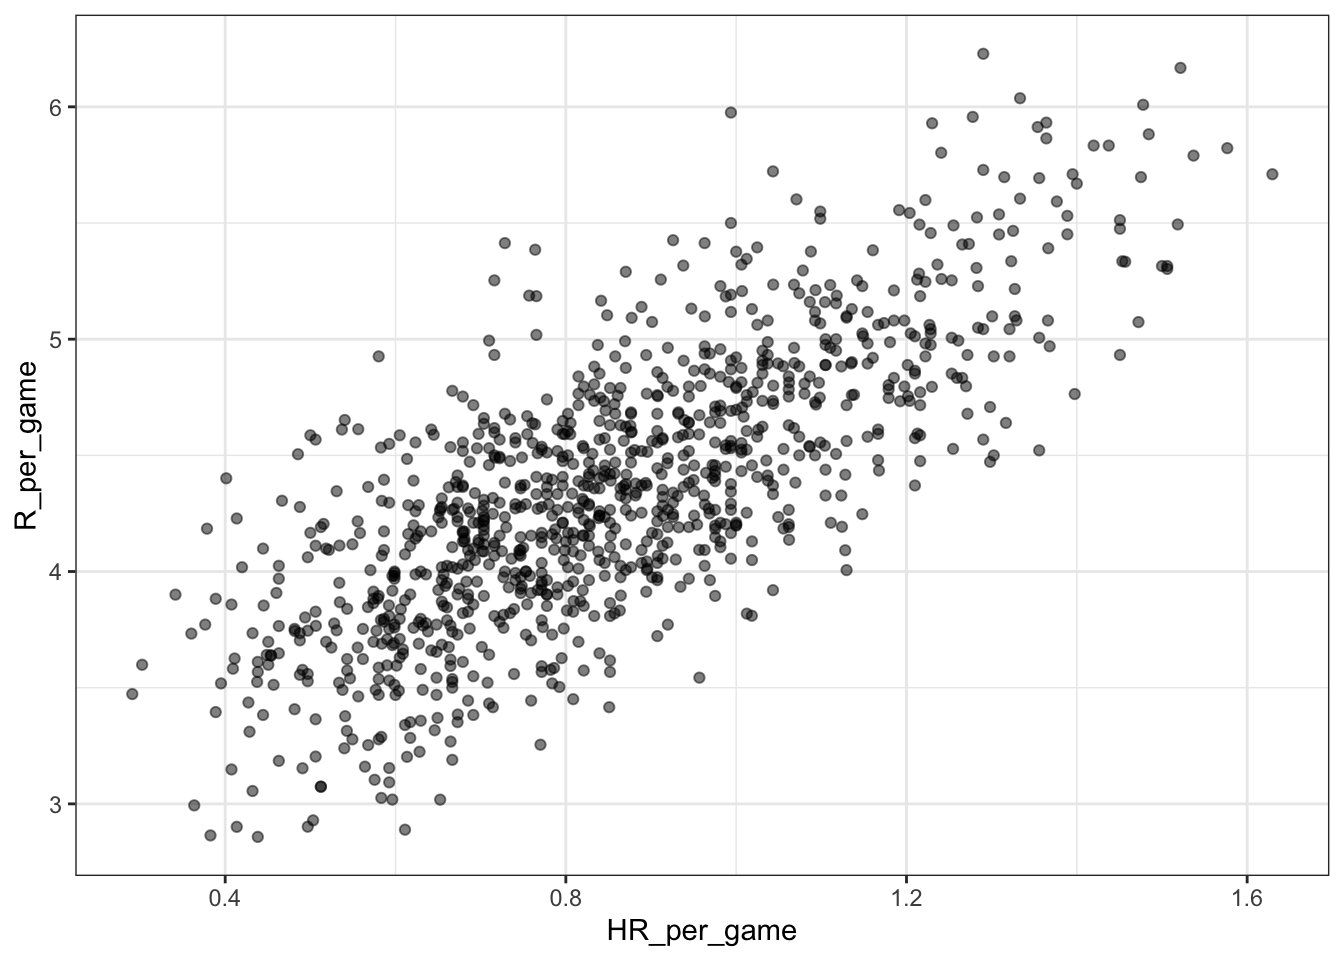
\includegraphics{Data_Science_Linear_Regression_files/figure-latex/unnamed-chunk-1-1.pdf}

\emph{Code: Scatterplot of the relationship between stolen bases and
runs}

\begin{Shaded}
\begin{Highlighting}[]
\NormalTok{Teams }\OperatorTok{\%\textgreater{}\%}\StringTok{ }\KeywordTok{filter}\NormalTok{(yearID }\OperatorTok{\%in\%}\StringTok{ }\DecValTok{1961}\OperatorTok{:}\DecValTok{2001}\NormalTok{) }\OperatorTok{\%\textgreater{}\%}
\StringTok{    }\KeywordTok{mutate}\NormalTok{(}\DataTypeTok{SB\_per\_game =}\NormalTok{ SB }\OperatorTok{/}\StringTok{ }\NormalTok{G, }\DataTypeTok{R\_per\_game =}\NormalTok{ R }\OperatorTok{/}\StringTok{ }\NormalTok{G) }\OperatorTok{\%\textgreater{}\%}
\StringTok{    }\KeywordTok{ggplot}\NormalTok{(}\KeywordTok{aes}\NormalTok{(SB\_per\_game, R\_per\_game)) }\OperatorTok{+}\StringTok{ }
\StringTok{    }\KeywordTok{geom\_point}\NormalTok{(}\DataTypeTok{alpha =} \FloatTok{0.5}\NormalTok{)}
\end{Highlighting}
\end{Shaded}

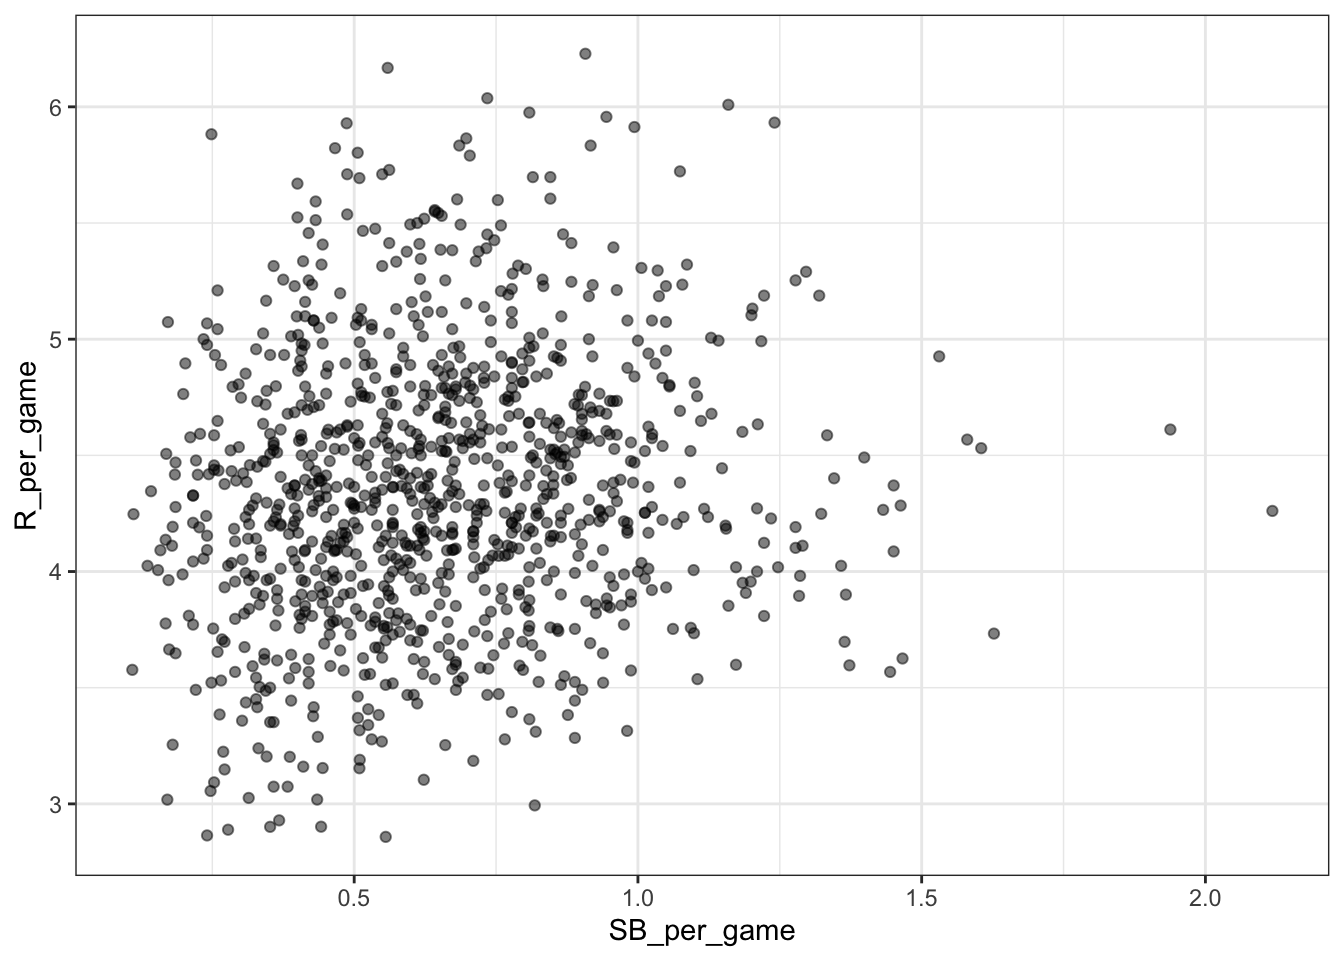
\includegraphics{Data_Science_Linear_Regression_files/figure-latex/unnamed-chunk-2-1.pdf}

\emph{Code: Scatterplot of the relationship between bases on balls and
runs}

\begin{Shaded}
\begin{Highlighting}[]
\NormalTok{Teams }\OperatorTok{\%\textgreater{}\%}\StringTok{ }\KeywordTok{filter}\NormalTok{(yearID }\OperatorTok{\%in\%}\StringTok{ }\DecValTok{1961}\OperatorTok{:}\DecValTok{2001}\NormalTok{) }\OperatorTok{\%\textgreater{}\%}
\StringTok{    }\KeywordTok{mutate}\NormalTok{(}\DataTypeTok{BB\_per\_game =}\NormalTok{ BB }\OperatorTok{/}\StringTok{ }\NormalTok{G, }\DataTypeTok{R\_per\_game =}\NormalTok{ R }\OperatorTok{/}\StringTok{ }\NormalTok{G) }\OperatorTok{\%\textgreater{}\%}
\StringTok{    }\KeywordTok{ggplot}\NormalTok{(}\KeywordTok{aes}\NormalTok{(BB\_per\_game, R\_per\_game)) }\OperatorTok{+}\StringTok{ }
\StringTok{    }\KeywordTok{geom\_point}\NormalTok{(}\DataTypeTok{alpha =} \FloatTok{0.5}\NormalTok{)}
\end{Highlighting}
\end{Shaded}

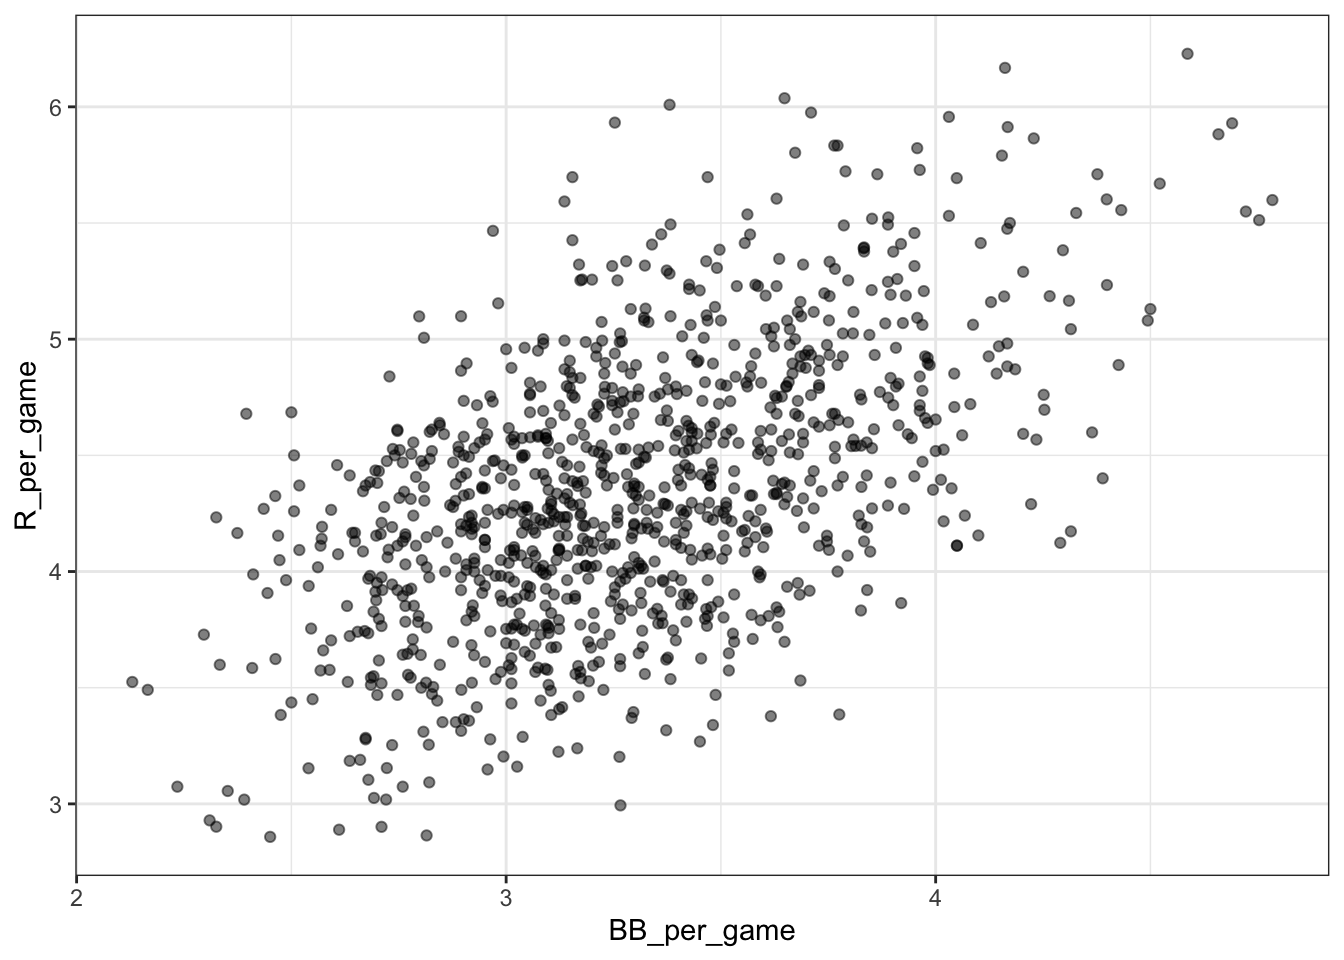
\includegraphics{Data_Science_Linear_Regression_files/figure-latex/unnamed-chunk-3-1.pdf}

\hypertarget{assessment---baseball-as-a-motivating-example}{%
\subsection{Assessment - Baseball as a Motivating
Example}\label{assessment---baseball-as-a-motivating-example}}

\begin{enumerate}
\def\labelenumi{\arabic{enumi}.}
\tightlist
\item
  What is the application of statistics and data science to baseball
  called?
\end{enumerate}

\begin{itemize}
\tightlist
\item[$\square$]
  A. Moneyball
\item[$\boxtimes$]
  B. Sabermetrics
\item[$\square$]
  C. The ``Oakland A's Approach''
\item[$\square$]
  D. There is no specific name for this; it's just data science.
\end{itemize}

\begin{enumerate}
\def\labelenumi{\arabic{enumi}.}
\setcounter{enumi}{1}
\tightlist
\item
  Which of the following outcomes is not included in the batting
  average?
\end{enumerate}

\begin{itemize}
\tightlist
\item[$\square$]
  A. A home run
\item[$\boxtimes$]
  B. A base on balls
\item[$\square$]
  C. An out
\item[$\square$]
  D. A single
\end{itemize}

\begin{enumerate}
\def\labelenumi{\arabic{enumi}.}
\setcounter{enumi}{2}
\tightlist
\item
  Why do we consider team statistics as well as individual player
  statistics?
\end{enumerate}

\begin{itemize}
\tightlist
\item[$\boxtimes$]
  A. The success of any individual player also depends on the strength
  of their team.
\item[$\square$]
  B. Team statistics can be easier to calculate.
\item[$\square$]
  C. The ultimate goal of sabermetrics is to rank teams, not players.
\end{itemize}

\begin{enumerate}
\def\labelenumi{\arabic{enumi}.}
\setcounter{enumi}{3}
\tightlist
\item
  You want to know whether teams with more at-bats per game have more
  runs per game. What R code below correctly makes a scatter plot for
  this relationship?
\end{enumerate}

\begin{Shaded}
\begin{Highlighting}[]
\NormalTok{Teams }\OperatorTok{\%\textgreater{}\%}\StringTok{ }\KeywordTok{filter}\NormalTok{(yearID }\OperatorTok{\%in\%}\StringTok{ }\DecValTok{1961}\OperatorTok{:}\DecValTok{2001}\NormalTok{ ) }\OperatorTok{\%\textgreater{}\%}
\StringTok{    }\KeywordTok{mutate}\NormalTok{(}\DataTypeTok{AB\_per\_game =}\NormalTok{ AB}\OperatorTok{/}\NormalTok{G, }\DataTypeTok{R\_per\_game =}\NormalTok{ R}\OperatorTok{/}\NormalTok{G) }\OperatorTok{\%\textgreater{}\%}
\StringTok{    }\KeywordTok{ggplot}\NormalTok{(}\KeywordTok{aes}\NormalTok{(AB\_per\_game, R\_per\_game)) }\OperatorTok{+}\StringTok{ }
\StringTok{    }\KeywordTok{geom\_point}\NormalTok{(}\DataTypeTok{alpha =} \FloatTok{0.5}\NormalTok{)}
\end{Highlighting}
\end{Shaded}

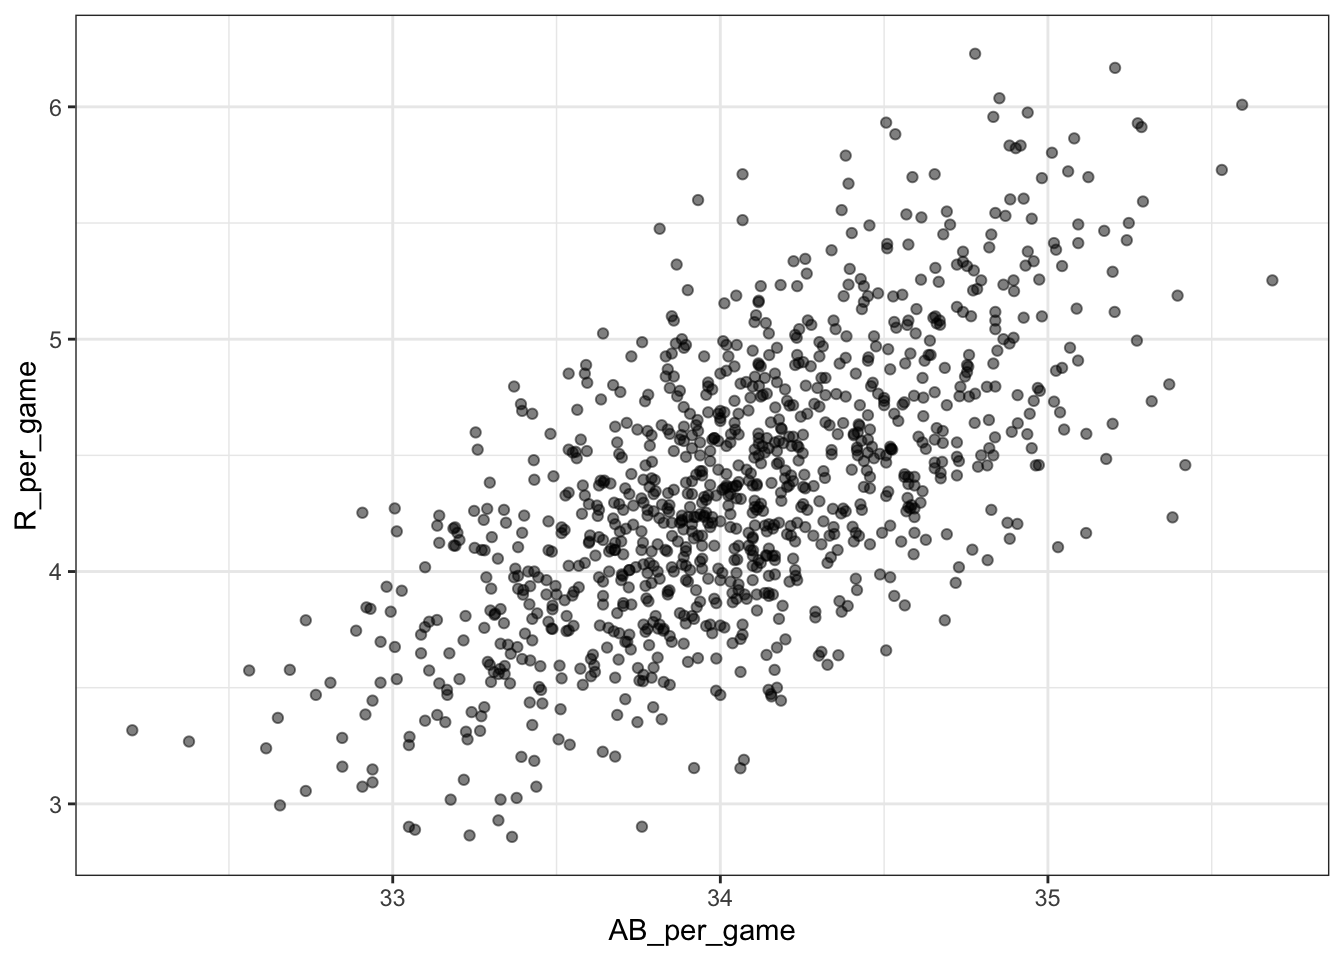
\includegraphics{Data_Science_Linear_Regression_files/figure-latex/unnamed-chunk-4-1.pdf}

\begin{itemize}
\tightlist
\item[$\square$]
  A.
\end{itemize}

\begin{Shaded}
\begin{Highlighting}[]
\NormalTok{Teams }\OperatorTok{\%\textgreater{}\%}\StringTok{ }\KeywordTok{filter}\NormalTok{(yearID }\OperatorTok{\%in\%}\StringTok{ }\DecValTok{1961}\OperatorTok{:}\DecValTok{2001}\NormalTok{ ) }\OperatorTok{\%\textgreater{}\%}
\StringTok{    }\KeywordTok{ggplot}\NormalTok{(}\KeywordTok{aes}\NormalTok{(AB, R)) }\OperatorTok{+}\StringTok{ }
\StringTok{    }\KeywordTok{geom\_point}\NormalTok{(}\DataTypeTok{alpha =} \FloatTok{0.5}\NormalTok{)}
\end{Highlighting}
\end{Shaded}

\begin{itemize}
\tightlist
\item[$\boxtimes$]
  B.
\end{itemize}

\begin{Shaded}
\begin{Highlighting}[]
\NormalTok{Teams }\OperatorTok{\%\textgreater{}\%}\StringTok{ }\KeywordTok{filter}\NormalTok{(yearID }\OperatorTok{\%in\%}\StringTok{ }\DecValTok{1961}\OperatorTok{:}\DecValTok{2001}\NormalTok{ ) }\OperatorTok{\%\textgreater{}\%}
\StringTok{    }\KeywordTok{mutate}\NormalTok{(}\DataTypeTok{AB\_per\_game =}\NormalTok{ AB}\OperatorTok{/}\NormalTok{G, }\DataTypeTok{R\_per\_game =}\NormalTok{ R}\OperatorTok{/}\NormalTok{G) }\OperatorTok{\%\textgreater{}\%}
\StringTok{    }\KeywordTok{ggplot}\NormalTok{(}\KeywordTok{aes}\NormalTok{(AB\_per\_game, R\_per\_game)) }\OperatorTok{+}\StringTok{ }
\StringTok{    }\KeywordTok{geom\_point}\NormalTok{(}\DataTypeTok{alpha =} \FloatTok{0.5}\NormalTok{)}
\end{Highlighting}
\end{Shaded}

\begin{itemize}
\tightlist
\item[$\square$]
  C.
\end{itemize}

\begin{Shaded}
\begin{Highlighting}[]
\NormalTok{Teams }\OperatorTok{\%\textgreater{}\%}\StringTok{ }\KeywordTok{filter}\NormalTok{(yearID }\OperatorTok{\%in\%}\StringTok{ }\DecValTok{1961}\OperatorTok{:}\DecValTok{2001}\NormalTok{ ) }\OperatorTok{\%\textgreater{}\%}
\StringTok{    }\KeywordTok{mutate}\NormalTok{(}\DataTypeTok{AB\_per\_game =}\NormalTok{ AB}\OperatorTok{/}\NormalTok{G, }\DataTypeTok{R\_per\_game =}\NormalTok{ R}\OperatorTok{/}\NormalTok{G) }\OperatorTok{\%\textgreater{}\%}
\StringTok{    }\KeywordTok{ggplot}\NormalTok{(}\KeywordTok{aes}\NormalTok{(AB\_per\_game, R\_per\_game)) }\OperatorTok{+}\StringTok{ }
\StringTok{    }\KeywordTok{geom\_line}\NormalTok{()}
\end{Highlighting}
\end{Shaded}

\begin{itemize}
\tightlist
\item[$\square$]
  D.
\end{itemize}

\begin{Shaded}
\begin{Highlighting}[]
\NormalTok{Teams }\OperatorTok{\%\textgreater{}\%}\StringTok{ }\KeywordTok{filter}\NormalTok{(yearID }\OperatorTok{\%in\%}\StringTok{ }\DecValTok{1961}\OperatorTok{:}\DecValTok{2001}\NormalTok{ ) }\OperatorTok{\%\textgreater{}\%}
\StringTok{    }\KeywordTok{mutate}\NormalTok{(}\DataTypeTok{AB\_per\_game =}\NormalTok{ AB}\OperatorTok{/}\NormalTok{G, }\DataTypeTok{R\_per\_game =}\NormalTok{ R}\OperatorTok{/}\NormalTok{G) }\OperatorTok{\%\textgreater{}\%}
\StringTok{    }\KeywordTok{ggplot}\NormalTok{(}\KeywordTok{aes}\NormalTok{(R\_per\_game, AB\_per\_game)) }\OperatorTok{+}\StringTok{ }
\StringTok{    }\KeywordTok{geom\_point}\NormalTok{()}
\end{Highlighting}
\end{Shaded}

\begin{enumerate}
\def\labelenumi{\arabic{enumi}.}
\setcounter{enumi}{4}
\tightlist
\item
  What does the variable ``SOA'' stand for in the Teams table?
\end{enumerate}

Hint: make sure to use the help file (\texttt{?Teams}).

\begin{itemize}
\tightlist
\item[$\square$]
  A. sacrifice out
\item[$\square$]
  B. slides or attempts
\item[$\boxtimes$]
  C. strikeouts by pitchers
\item[$\square$]
  D. accumulated singles
\end{itemize}

\begin{enumerate}
\def\labelenumi{\arabic{enumi}.}
\setcounter{enumi}{5}
\tightlist
\item
  Load the \textbf{Lahman} library. Filter the \texttt{Teams} data frame
  to include years from 1961 to 2001. Make a scatterplot of runs per
  game versus at bats (\texttt{AB}) per game.
\end{enumerate}

\begin{Shaded}
\begin{Highlighting}[]
\NormalTok{Teams }\OperatorTok{\%\textgreater{}\%}\StringTok{ }\KeywordTok{filter}\NormalTok{(yearID }\OperatorTok{\%in\%}\StringTok{ }\DecValTok{1961}\OperatorTok{:}\DecValTok{2001}\NormalTok{) }\OperatorTok{\%\textgreater{}\%}
\StringTok{  }\KeywordTok{mutate}\NormalTok{(}\DataTypeTok{AB\_per\_game =}\NormalTok{ AB }\OperatorTok{/}\StringTok{ }\NormalTok{G, }\DataTypeTok{R\_per\_game =}\NormalTok{ R }\OperatorTok{/}\StringTok{ }\NormalTok{G) }\OperatorTok{\%\textgreater{}\%}
\StringTok{  }\KeywordTok{ggplot}\NormalTok{(}\KeywordTok{aes}\NormalTok{(AB\_per\_game, R\_per\_game)) }\OperatorTok{+}\StringTok{ }
\StringTok{  }\KeywordTok{geom\_point}\NormalTok{(}\DataTypeTok{alpha =} \FloatTok{0.5}\NormalTok{)}
\end{Highlighting}
\end{Shaded}

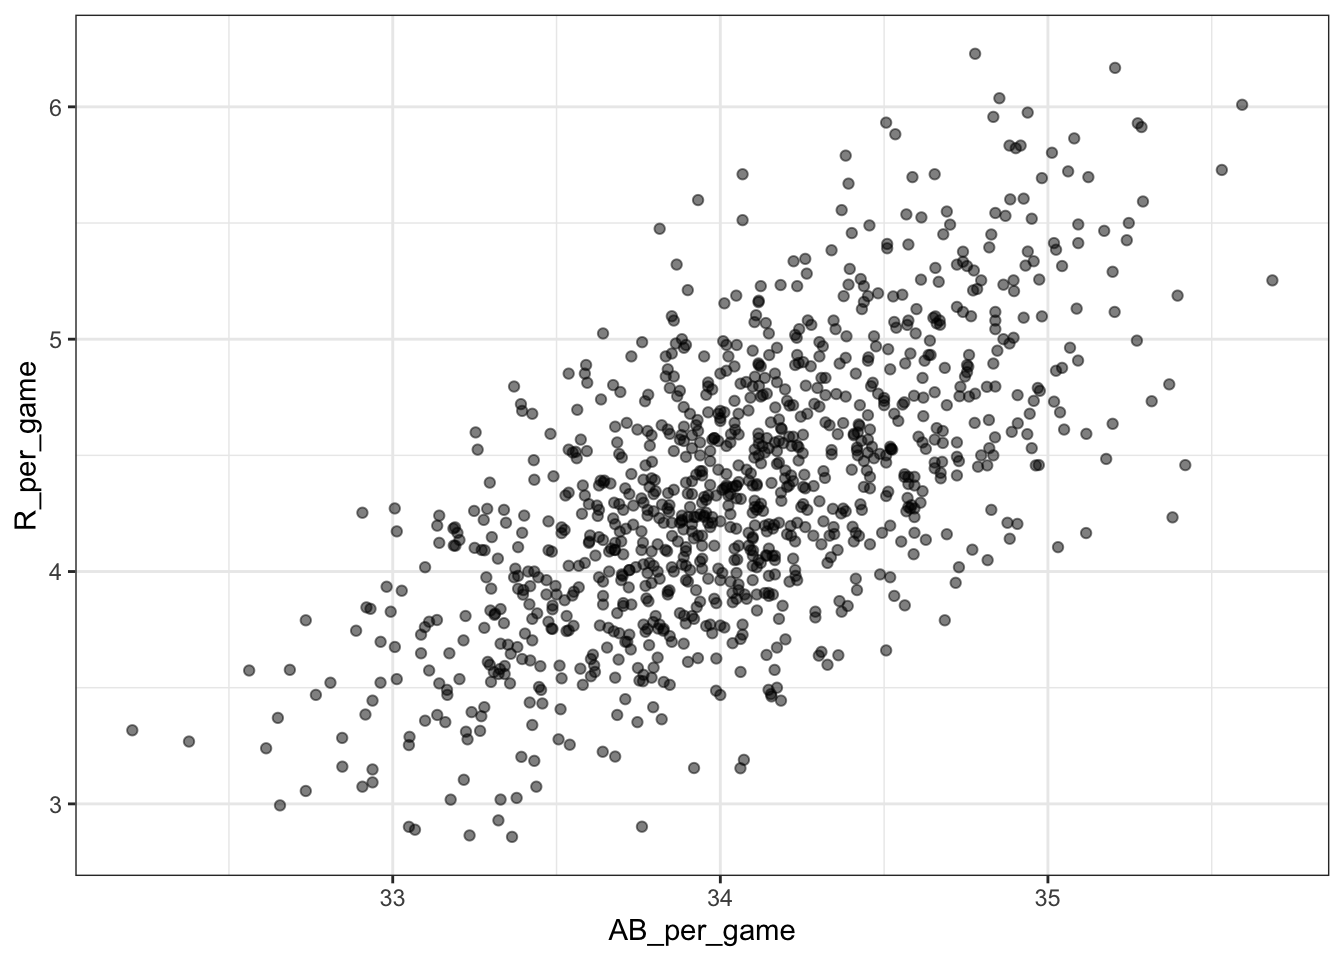
\includegraphics{Data_Science_Linear_Regression_files/figure-latex/unnamed-chunk-9-1.pdf}

Which of the following is true?

\begin{itemize}
\tightlist
\item[$\square$]
  A. There is no clear relationship between runs and at bats per game.
\item[$\boxtimes$]
  B. As the number of at bats per game increases, the number of runs per
  game tends to increase.
\item[$\square$]
  C. As the number of at bats per game increases, the number of runs per
  game tends to decrease.
\end{itemize}

\begin{enumerate}
\def\labelenumi{\arabic{enumi}.}
\setcounter{enumi}{6}
\tightlist
\item
  Use the filtered \texttt{Teams} data frame from Question 6. Make a
  scatterplot of win rate (number of wins per game) versus number of
  fielding errors (\texttt{E}) per game.
\end{enumerate}

\begin{Shaded}
\begin{Highlighting}[]
\NormalTok{Teams }\OperatorTok{\%\textgreater{}\%}\StringTok{ }\KeywordTok{filter}\NormalTok{(yearID }\OperatorTok{\%in\%}\StringTok{ }\DecValTok{1961}\OperatorTok{:}\DecValTok{2001}\NormalTok{) }\OperatorTok{\%\textgreater{}\%}
\StringTok{  }\KeywordTok{mutate}\NormalTok{(}\DataTypeTok{win\_rate =}\NormalTok{ W }\OperatorTok{/}\StringTok{ }\NormalTok{G, }\DataTypeTok{E\_per\_game =}\NormalTok{ E }\OperatorTok{/}\StringTok{ }\NormalTok{G) }\OperatorTok{\%\textgreater{}\%}
\StringTok{  }\KeywordTok{ggplot}\NormalTok{(}\KeywordTok{aes}\NormalTok{(win\_rate, E\_per\_game)) }\OperatorTok{+}\StringTok{ }
\StringTok{  }\KeywordTok{geom\_point}\NormalTok{(}\DataTypeTok{alpha =} \FloatTok{0.5}\NormalTok{)}
\end{Highlighting}
\end{Shaded}

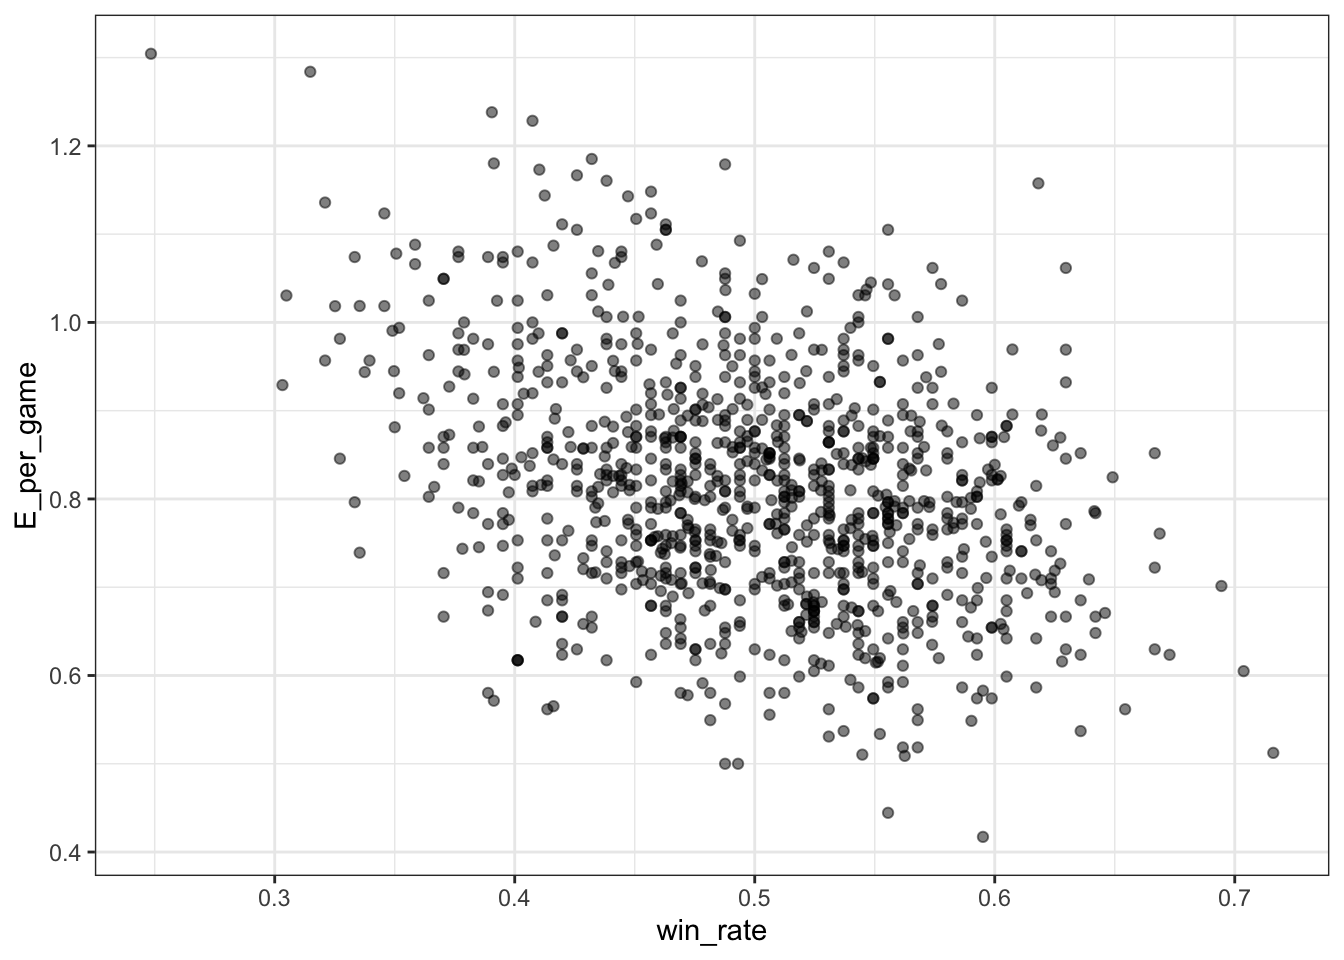
\includegraphics{Data_Science_Linear_Regression_files/figure-latex/unnamed-chunk-10-1.pdf}

Which of the following is true?

\begin{itemize}
\tightlist
\item[$\square$]
  A. There is no relationship between win rate and errors per game.
\item[$\square$]
  B. As the number of errors per game increases, the win rate tends to
  increase.
\item[$\boxtimes$]
  C. As the number of errors per game increases, the win rate tends to
  decrease.
\end{itemize}

\begin{enumerate}
\def\labelenumi{\arabic{enumi}.}
\setcounter{enumi}{7}
\tightlist
\item
  Use the filtered \texttt{Teams} data frame from Question 6. Make a
  scatterplot of triples (\texttt{X3B}) per game versus doubles
  (\texttt{X2B}) per game.
\end{enumerate}

\begin{Shaded}
\begin{Highlighting}[]
\NormalTok{Teams }\OperatorTok{\%\textgreater{}\%}\StringTok{ }\KeywordTok{filter}\NormalTok{(yearID }\OperatorTok{\%in\%}\StringTok{ }\DecValTok{1961}\OperatorTok{:}\DecValTok{2001}\NormalTok{) }\OperatorTok{\%\textgreater{}\%}
\StringTok{  }\KeywordTok{mutate}\NormalTok{(}\DataTypeTok{doubles\_per\_game =}\NormalTok{ X2B }\OperatorTok{/}\StringTok{ }\NormalTok{G, }\DataTypeTok{triples\_per\_game =}\NormalTok{ X3B }\OperatorTok{/}\StringTok{ }\NormalTok{G) }\OperatorTok{\%\textgreater{}\%}
\StringTok{  }\KeywordTok{ggplot}\NormalTok{(}\KeywordTok{aes}\NormalTok{(doubles\_per\_game, triples\_per\_game)) }\OperatorTok{+}\StringTok{ }
\StringTok{  }\KeywordTok{geom\_point}\NormalTok{(}\DataTypeTok{alpha =} \FloatTok{0.5}\NormalTok{)}
\end{Highlighting}
\end{Shaded}

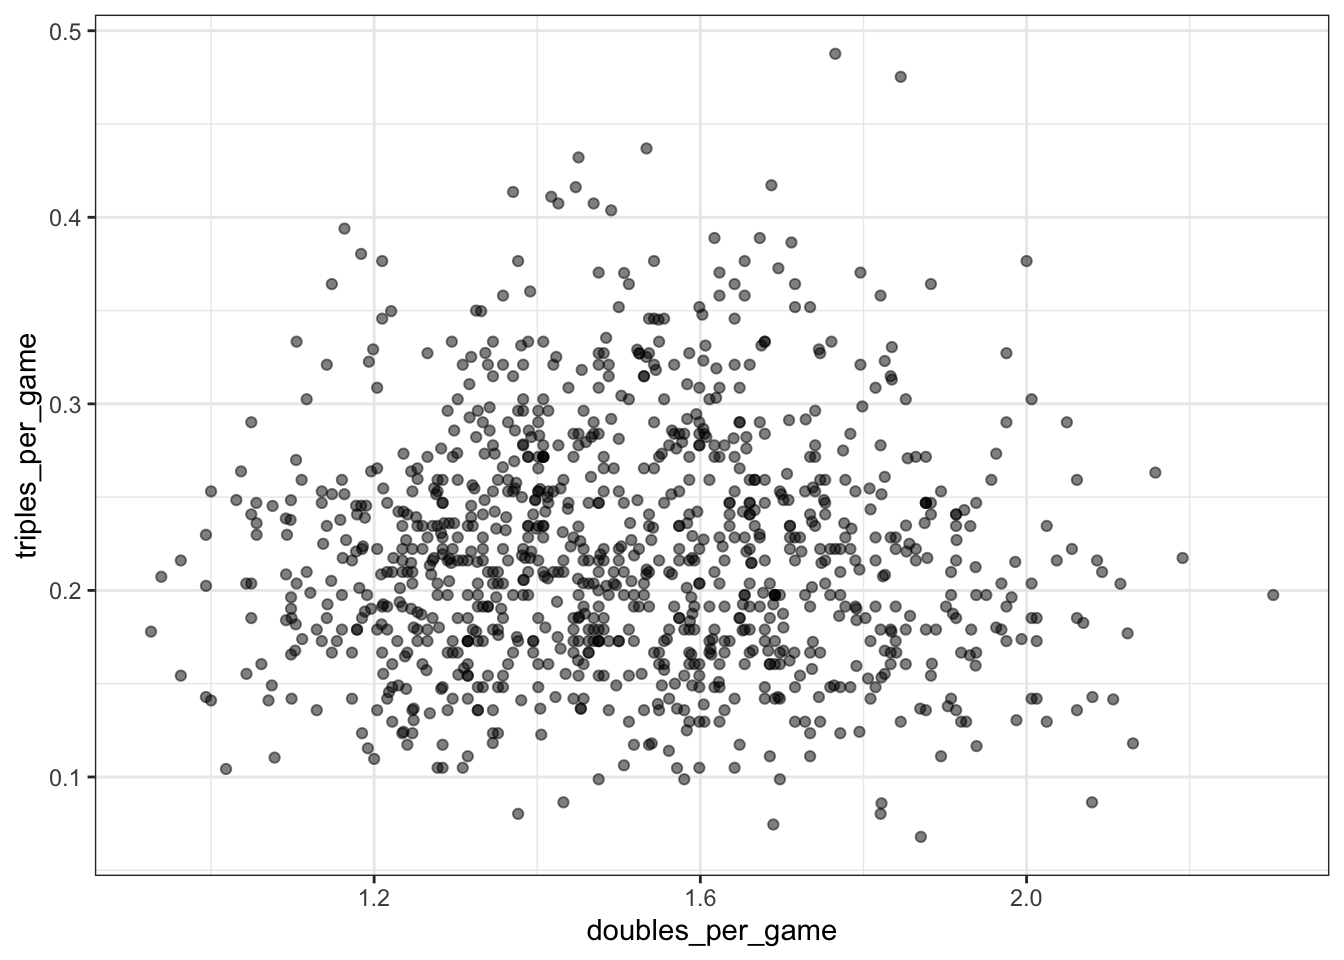
\includegraphics{Data_Science_Linear_Regression_files/figure-latex/unnamed-chunk-11-1.pdf}

Which of the following is true?

\begin{itemize}
\tightlist
\item[$\boxtimes$]
  A. There is no clear relationship between doubles per game and triples
  per game.
\item[$\square$]
  B. As the number of doubles per game increases, the number of triples
  per game tends to increase.
\item[$\square$]
  C. As the number of doubles per game increases, the number of triples
  per game tends to decrease.
\end{itemize}

\hypertarget{correlation}{%
\subsection{Correlation}\label{correlation}}

The corresponding textbook section is
\href{https://rafalab.github.io/dsbook/regression.html\#case-study-is-height-hereditary}{Case
Study: is height hereditary?}

\textbf{Key points}

\begin{itemize}
\tightlist
\item
  Galton tried to predict sons' heights based on fathers' heights.
\item
  The mean and standard errors are insufficient for describing an
  important characteristic of the data: the trend that the taller the
  father, the taller the son.
\item
  The correlation coefficient is an informative summary of how two
  variables move together that can be used to predict one variable using
  the other.
\end{itemize}

\emph{Code}

\begin{Shaded}
\begin{Highlighting}[]
\CommentTok{\# create the dataset}
\ControlFlowTok{if}\NormalTok{(}\OperatorTok{!}\KeywordTok{require}\NormalTok{(HistData)) }\KeywordTok{install.packages}\NormalTok{(}\StringTok{"HistData"}\NormalTok{)}
\end{Highlighting}
\end{Shaded}

\begin{verbatim}
## Loading required package: HistData
\end{verbatim}

\begin{Shaded}
\begin{Highlighting}[]
\KeywordTok{library}\NormalTok{(tidyverse)}
\KeywordTok{library}\NormalTok{(HistData)}
\KeywordTok{data}\NormalTok{(}\StringTok{"GaltonFamilies"}\NormalTok{)}
\KeywordTok{set.seed}\NormalTok{(}\DecValTok{1983}\NormalTok{)}
\NormalTok{galton\_heights \textless{}{-}}\StringTok{ }\NormalTok{GaltonFamilies }\OperatorTok{\%\textgreater{}\%}
\StringTok{  }\KeywordTok{filter}\NormalTok{(gender }\OperatorTok{==}\StringTok{ "male"}\NormalTok{) }\OperatorTok{\%\textgreater{}\%}
\StringTok{  }\KeywordTok{group\_by}\NormalTok{(family) }\OperatorTok{\%\textgreater{}\%}
\StringTok{  }\KeywordTok{sample\_n}\NormalTok{(}\DecValTok{1}\NormalTok{) }\OperatorTok{\%\textgreater{}\%}
\StringTok{  }\KeywordTok{ungroup}\NormalTok{() }\OperatorTok{\%\textgreater{}\%}
\StringTok{  }\KeywordTok{select}\NormalTok{(father, childHeight) }\OperatorTok{\%\textgreater{}\%}
\StringTok{  }\KeywordTok{rename}\NormalTok{(}\DataTypeTok{son =}\NormalTok{ childHeight)}

\CommentTok{\# means and standard deviations}
\NormalTok{galton\_heights }\OperatorTok{\%\textgreater{}\%}
\StringTok{    }\KeywordTok{summarize}\NormalTok{(}\KeywordTok{mean}\NormalTok{(father), }\KeywordTok{sd}\NormalTok{(father), }\KeywordTok{mean}\NormalTok{(son), }\KeywordTok{sd}\NormalTok{(son))}
\end{Highlighting}
\end{Shaded}

\begin{verbatim}
## # A tibble: 1 x 4
##   `mean(father)` `sd(father)` `mean(son)` `sd(son)`
##            <dbl>        <dbl>       <dbl>     <dbl>
## 1           69.1         2.55        69.2      2.71
\end{verbatim}

\begin{Shaded}
\begin{Highlighting}[]
\CommentTok{\# scatterplot of father and son heights}
\NormalTok{galton\_heights }\OperatorTok{\%\textgreater{}\%}
\StringTok{    }\KeywordTok{ggplot}\NormalTok{(}\KeywordTok{aes}\NormalTok{(father, son)) }\OperatorTok{+}
\StringTok{    }\KeywordTok{geom\_point}\NormalTok{(}\DataTypeTok{alpha =} \FloatTok{0.5}\NormalTok{)}
\end{Highlighting}
\end{Shaded}

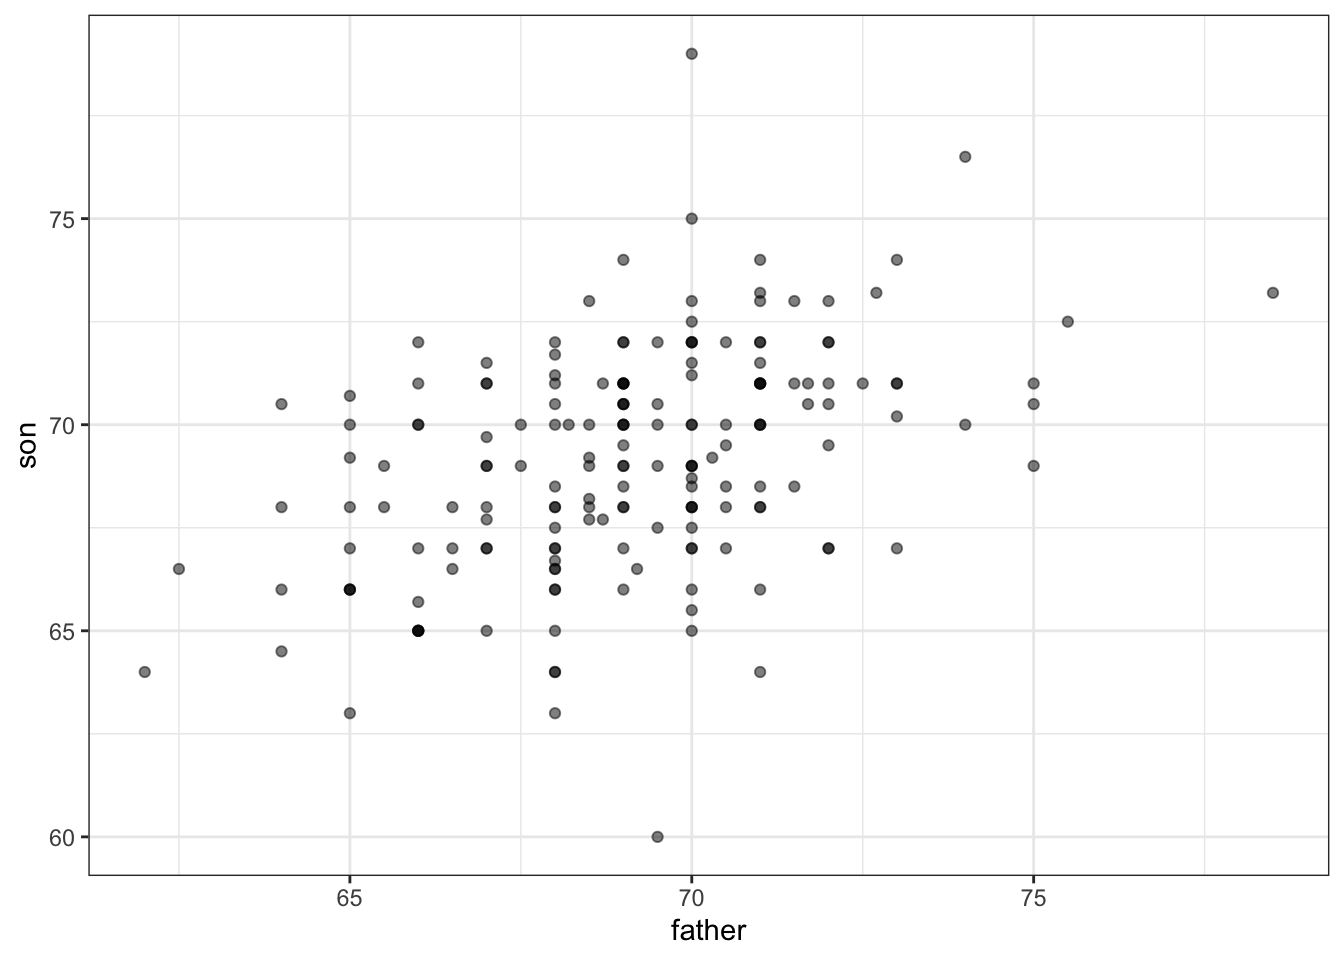
\includegraphics{Data_Science_Linear_Regression_files/figure-latex/unnamed-chunk-12-1.pdf}

\hypertarget{correlation-coefficient}{%
\subsection{Correlation Coefficient}\label{correlation-coefficient}}

The corresponding textbook section is
\href{https://rafalab.github.io/dsbook/regression.html\#corr-coef}{the
correlation coefficient}

\textbf{Key points}

\begin{itemize}
\tightlist
\item
  The correlation coefficient is defined for a list of pairs
  \((x_1, y_1), ..., (x_n, y_n)\) as the product of the standardized
  values:
  \((\frac{x_i - \mu_x}{\sigma_x})(\frac{y_i -\mu_y}{\sigma_y})\).
\item
  The correlation coefficient essentially conveys how two variables move
  together.
\item
  The correlation coefficient is always between -1 and 1.
\end{itemize}

\emph{Code}

\begin{Shaded}
\begin{Highlighting}[]
\NormalTok{rho \textless{}{-}}\StringTok{ }\KeywordTok{mean}\NormalTok{(}\KeywordTok{scale}\NormalTok{(x)}\OperatorTok{*}\KeywordTok{scale}\NormalTok{(y))}
\end{Highlighting}
\end{Shaded}

\begin{Shaded}
\begin{Highlighting}[]
\KeywordTok{data}\NormalTok{(}\StringTok{"GaltonFamilies"}\NormalTok{)}
\NormalTok{galton\_heights \textless{}{-}}\StringTok{ }\NormalTok{GaltonFamilies }\OperatorTok{\%\textgreater{}\%}\StringTok{ }\KeywordTok{filter}\NormalTok{(childNum }\OperatorTok{==}\StringTok{ }\DecValTok{1} \OperatorTok{\&}\StringTok{ }\NormalTok{gender }\OperatorTok{==}\StringTok{ "male"}\NormalTok{) }\OperatorTok{\%\textgreater{}\%}\StringTok{ }\KeywordTok{select}\NormalTok{(father, childHeight) }\OperatorTok{\%\textgreater{}\%}\StringTok{ }\KeywordTok{rename}\NormalTok{(}\DataTypeTok{son =}\NormalTok{ childHeight)}
\NormalTok{galton\_heights }\OperatorTok{\%\textgreater{}\%}\StringTok{ }\KeywordTok{summarize}\NormalTok{(}\DataTypeTok{r =} \KeywordTok{cor}\NormalTok{(father, son)) }\OperatorTok{\%\textgreater{}\%}\StringTok{ }\KeywordTok{pull}\NormalTok{(r)}
\end{Highlighting}
\end{Shaded}

\begin{verbatim}
## [1] 0.5007248
\end{verbatim}

\hypertarget{sample-correlation-is-a-random-variable}{%
\subsection{Sample Correlation is a Random
Variable}\label{sample-correlation-is-a-random-variable}}

The corresponding textbook section is
\href{https://rafalab.github.io/dsbook/regression.html\#sample-correlation-is-a-random-variable}{Sample
correlation is a random variable}

\textbf{Key points}

\begin{itemize}
\tightlist
\item
  The correlation that we compute and use as a summary is a random
  variable.
\item
  When interpreting correlations, it is important to remember that
  correlations derived from samples are estimates containing
  uncertainty.
\item
  Because the sample correlation is an average of independent draws, the
  central limit theorem applies.
\end{itemize}

\emph{Code}

\begin{Shaded}
\begin{Highlighting}[]
\CommentTok{\# compute sample correlation}
\NormalTok{R \textless{}{-}}\StringTok{ }\KeywordTok{sample\_n}\NormalTok{(galton\_heights, }\DecValTok{25}\NormalTok{, }\DataTypeTok{replace =} \OtherTok{TRUE}\NormalTok{) }\OperatorTok{\%\textgreater{}\%}
\StringTok{    }\KeywordTok{summarize}\NormalTok{(}\DataTypeTok{r =} \KeywordTok{cor}\NormalTok{(father, son))}
\NormalTok{R}
\end{Highlighting}
\end{Shaded}

\begin{verbatim}
##           r
## 1 0.4787613
\end{verbatim}

\begin{Shaded}
\begin{Highlighting}[]
\CommentTok{\# Monte Carlo simulation to show distribution of sample correlation}
\NormalTok{B \textless{}{-}}\StringTok{ }\DecValTok{1000}
\NormalTok{N \textless{}{-}}\StringTok{ }\DecValTok{25}
\NormalTok{R \textless{}{-}}\StringTok{ }\KeywordTok{replicate}\NormalTok{(B, \{}
    \KeywordTok{sample\_n}\NormalTok{(galton\_heights, N, }\DataTypeTok{replace =} \OtherTok{TRUE}\NormalTok{) }\OperatorTok{\%\textgreater{}\%}
\StringTok{    }\KeywordTok{summarize}\NormalTok{(}\DataTypeTok{r =} \KeywordTok{cor}\NormalTok{(father, son)) }\OperatorTok{\%\textgreater{}\%}
\StringTok{    }\KeywordTok{pull}\NormalTok{(r)}
\NormalTok{\})}
\KeywordTok{qplot}\NormalTok{(R, }\DataTypeTok{geom =} \StringTok{"histogram"}\NormalTok{, }\DataTypeTok{binwidth =} \FloatTok{0.05}\NormalTok{, }\DataTypeTok{color =} \KeywordTok{I}\NormalTok{(}\StringTok{"black"}\NormalTok{))}
\end{Highlighting}
\end{Shaded}

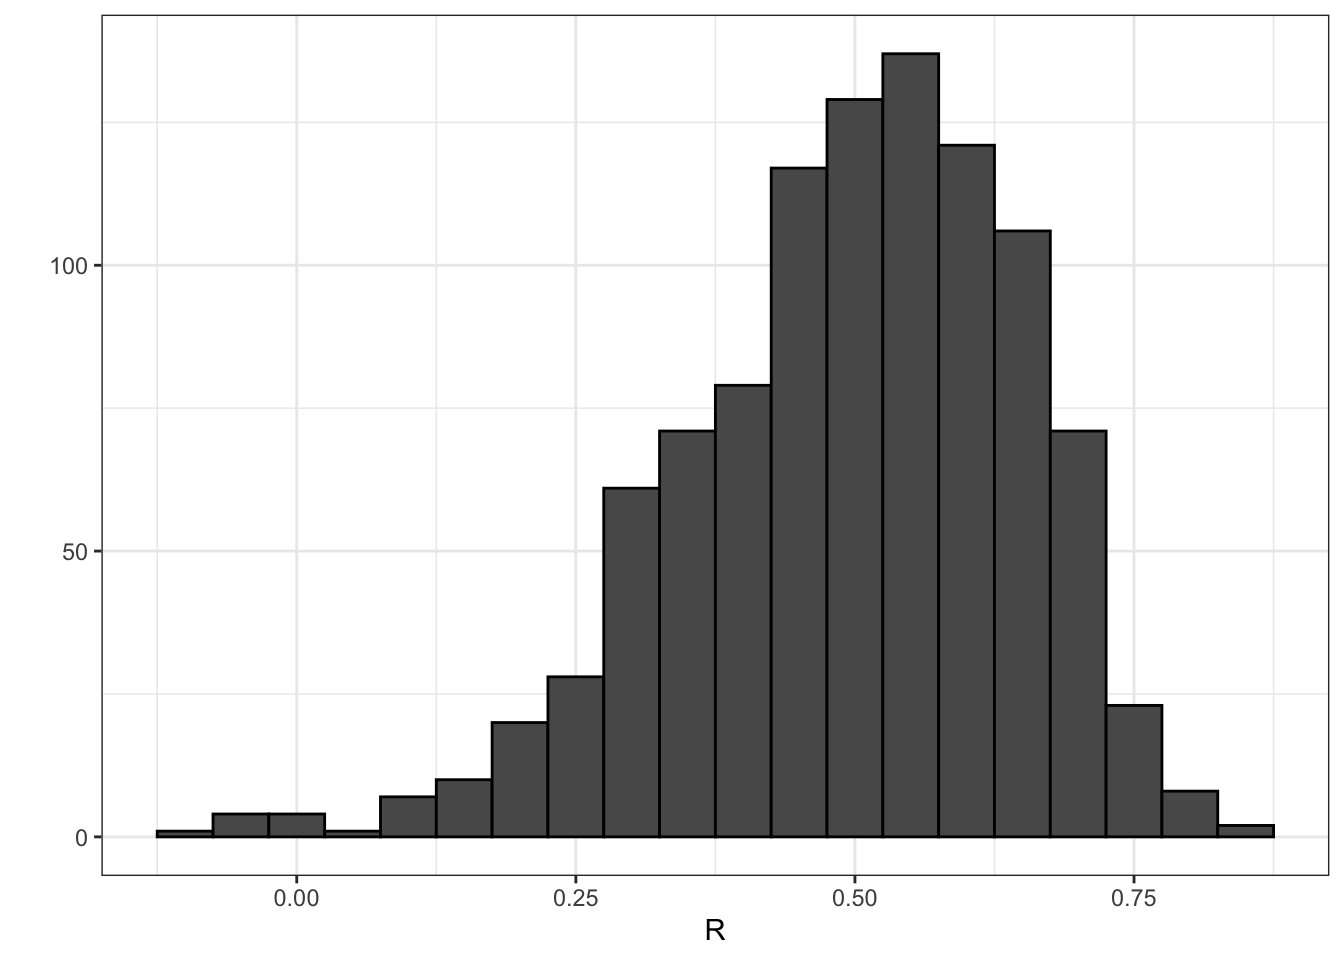
\includegraphics{Data_Science_Linear_Regression_files/figure-latex/unnamed-chunk-15-1.pdf}

\begin{Shaded}
\begin{Highlighting}[]
\CommentTok{\# expected value and standard error}
\KeywordTok{mean}\NormalTok{(R)}
\end{Highlighting}
\end{Shaded}

\begin{verbatim}
## [1] 0.4970997
\end{verbatim}

\begin{Shaded}
\begin{Highlighting}[]
\KeywordTok{sd}\NormalTok{(R)}
\end{Highlighting}
\end{Shaded}

\begin{verbatim}
## [1] 0.1512451
\end{verbatim}

\begin{Shaded}
\begin{Highlighting}[]
\CommentTok{\# QQ{-}plot to evaluate whether N is large enough}
\KeywordTok{data.frame}\NormalTok{(R) }\OperatorTok{\%\textgreater{}\%}
\StringTok{    }\KeywordTok{ggplot}\NormalTok{(}\KeywordTok{aes}\NormalTok{(}\DataTypeTok{sample =}\NormalTok{ R)) }\OperatorTok{+}
\StringTok{    }\KeywordTok{stat\_qq}\NormalTok{() }\OperatorTok{+}
\StringTok{    }\KeywordTok{geom\_abline}\NormalTok{(}\DataTypeTok{intercept =} \KeywordTok{mean}\NormalTok{(R), }\DataTypeTok{slope =} \KeywordTok{sqrt}\NormalTok{((}\DecValTok{1}\OperatorTok{{-}}\KeywordTok{mean}\NormalTok{(R)}\OperatorTok{\^{}}\DecValTok{2}\NormalTok{)}\OperatorTok{/}\NormalTok{(N}\DecValTok{{-}2}\NormalTok{)))}
\end{Highlighting}
\end{Shaded}

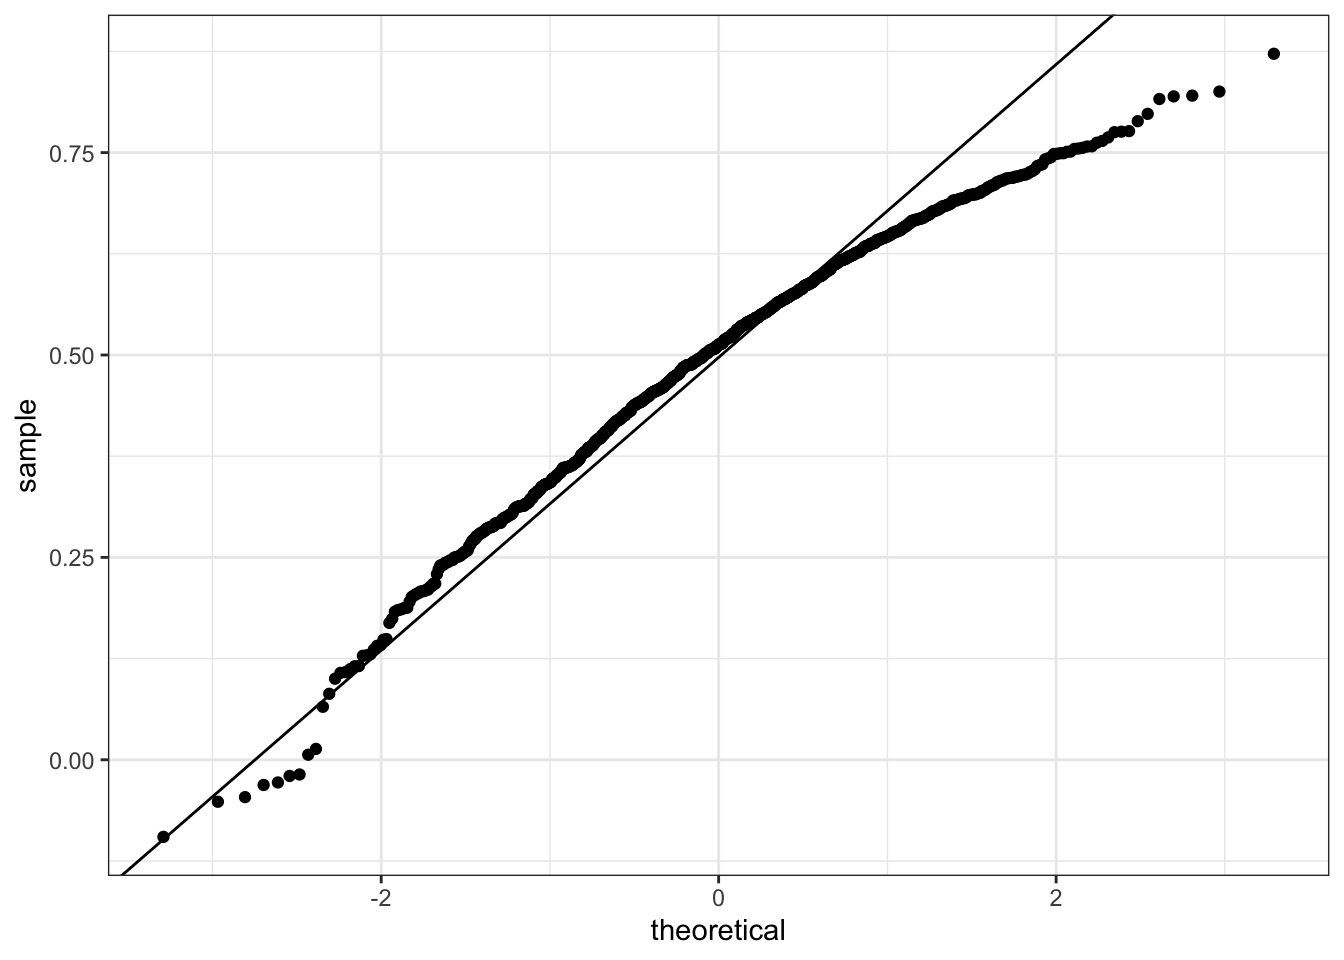
\includegraphics{Data_Science_Linear_Regression_files/figure-latex/unnamed-chunk-15-2.pdf}

\hypertarget{assessment---correlation}{%
\subsection{Assessment - Correlation}\label{assessment---correlation}}

\begin{enumerate}
\def\labelenumi{\arabic{enumi}.}
\tightlist
\item
  While studying heredity, Francis Galton developed what important
  statistical concept?
\end{enumerate}

\begin{itemize}
\tightlist
\item[$\square$]
  A. Standard deviation
\item[$\square$]
  B. Normal distribution
\item[$\boxtimes$]
  C. Correlation
\item[$\square$]
  D. Probability
\end{itemize}

\begin{enumerate}
\def\labelenumi{\arabic{enumi}.}
\setcounter{enumi}{1}
\tightlist
\item
  The correlation coefficient is a summary of what?
\end{enumerate}

\begin{itemize}
\tightlist
\item[$\boxtimes$]
  A. The trend between two variables
\item[$\square$]
  B. The dispersion of a variable
\item[$\square$]
  C. The central tendency of a variable
\item[$\square$]
  D. The distribution of a variable
\end{itemize}

\begin{enumerate}
\def\labelenumi{\arabic{enumi}.}
\setcounter{enumi}{2}
\tightlist
\item
  Below is a scatter plot showing the relationship between two
  variables, x and y.
\end{enumerate}

\begin{figure}
\centering
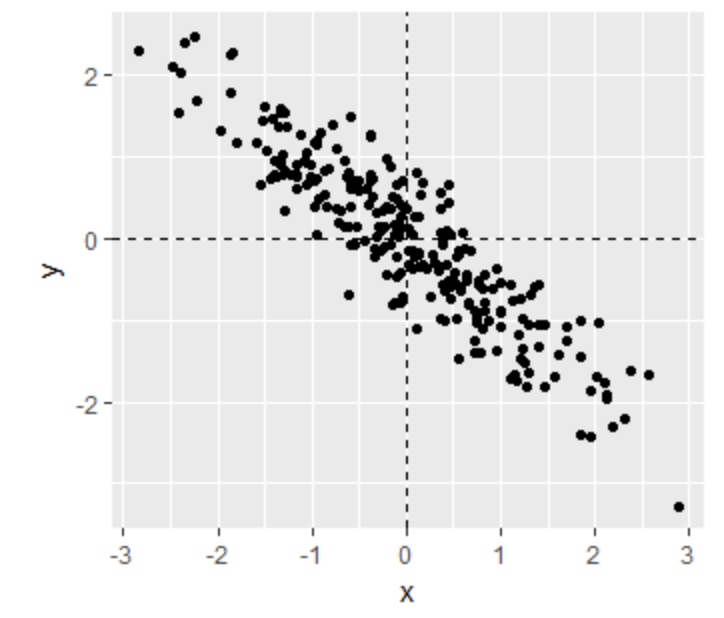
\includegraphics{images/scatterplot_x_y.png}
\caption{Scatter plot relationship x and y}
\end{figure}

From this figure, the correlation between x and y appears to be about:

\begin{itemize}
\tightlist
\item[$\boxtimes$]
  A. -0.9
\item[$\square$]
  B. -0.2
\item[$\square$]
  C. 0.9
\item[$\square$]
  D. 2
\end{itemize}

\begin{enumerate}
\def\labelenumi{\arabic{enumi}.}
\setcounter{enumi}{3}
\tightlist
\item
  Instead of running a Monte Carlo simulation with a sample size of 25
  from our 179 father-son pairs, we now run our simulation with a sample
  size of 50.
\end{enumerate}

Would you expect the \textbf{mean} of our sample correlation to
increase, decrease, or stay approximately the same?

\begin{itemize}
\tightlist
\item[$\square$]
  A. Increase
\item[$\square$]
  B. Decrease
\item[$\boxtimes$]
  C. Stay approximately the same
\end{itemize}

\begin{enumerate}
\def\labelenumi{\arabic{enumi}.}
\setcounter{enumi}{4}
\tightlist
\item
  Instead of running a Monte Carlo simulation with a sample size of 25
  from our 179 father-son pairs, we now run our simulation with a sample
  size of 50.
\end{enumerate}

Would you expect the \textbf{standard deviation} of our sample
correlation to increase, decrease, or stay approximately the same?

\begin{itemize}
\tightlist
\item[$\square$]
  A. Increase
\item[$\boxtimes$]
  B. Decrease
\item[$\square$]
  C. Stay approximately the same
\end{itemize}

\begin{enumerate}
\def\labelenumi{\arabic{enumi}.}
\setcounter{enumi}{5}
\tightlist
\item
  If X and Y are completely independent, what do you expect the value of
  the correlation coefficient to be?
\end{enumerate}

\begin{itemize}
\tightlist
\item[$\square$]
  A. -1
\item[$\square$]
  B. -0.5
\item[$\boxtimes$]
  C. 0
\item[$\square$]
  D. 0.5
\item[$\square$]
  E. 1
\item[$\square$]
  F. Not enough information to answer the question
\end{itemize}

\begin{enumerate}
\def\labelenumi{\arabic{enumi}.}
\setcounter{enumi}{6}
\tightlist
\item
  Load the \textbf{Lahman} library. Filter the \texttt{Teams} data frame
  to include years from 1961 to 2001.
\end{enumerate}

What is the correlation coefficient between number of runs per game and
number of at bats per game?

\begin{Shaded}
\begin{Highlighting}[]
\KeywordTok{library}\NormalTok{(Lahman)}
\NormalTok{Teams\_small \textless{}{-}}\StringTok{ }\NormalTok{Teams }\OperatorTok{\%\textgreater{}\%}\StringTok{ }\KeywordTok{filter}\NormalTok{(yearID }\OperatorTok{\%in\%}\StringTok{ }\DecValTok{1961}\OperatorTok{:}\DecValTok{2001}\NormalTok{)}
\KeywordTok{cor}\NormalTok{(Teams\_small}\OperatorTok{$}\NormalTok{R}\OperatorTok{/}\NormalTok{Teams\_small}\OperatorTok{$}\NormalTok{G, Teams\_small}\OperatorTok{$}\NormalTok{AB}\OperatorTok{/}\NormalTok{Teams\_small}\OperatorTok{$}\NormalTok{G)}
\end{Highlighting}
\end{Shaded}

\begin{verbatim}
## [1] 0.6580976
\end{verbatim}

\begin{enumerate}
\def\labelenumi{\arabic{enumi}.}
\setcounter{enumi}{7}
\tightlist
\item
  Use the filtered \texttt{Teams} data frame from Question 7.
\end{enumerate}

What is the correlation coefficient between win rate (number of wins per
game) and number of errors per game?

\begin{Shaded}
\begin{Highlighting}[]
\KeywordTok{cor}\NormalTok{(Teams\_small}\OperatorTok{$}\NormalTok{W}\OperatorTok{/}\NormalTok{Teams\_small}\OperatorTok{$}\NormalTok{G, Teams\_small}\OperatorTok{$}\NormalTok{E}\OperatorTok{/}\NormalTok{Teams\_small}\OperatorTok{$}\NormalTok{G)}
\end{Highlighting}
\end{Shaded}

\begin{verbatim}
## [1] -0.3396947
\end{verbatim}

\begin{enumerate}
\def\labelenumi{\arabic{enumi}.}
\setcounter{enumi}{8}
\tightlist
\item
  Use the filtered \texttt{Teams} data frame from Question 7.
\end{enumerate}

What is the correlation coefficient between doubles (\texttt{X2B}) per
game and triples (\texttt{X3B}) per game?

\begin{Shaded}
\begin{Highlighting}[]
\KeywordTok{cor}\NormalTok{(Teams\_small}\OperatorTok{$}\NormalTok{X2B}\OperatorTok{/}\NormalTok{Teams\_small}\OperatorTok{$}\NormalTok{G, Teams\_small}\OperatorTok{$}\NormalTok{X3B}\OperatorTok{/}\NormalTok{Teams\_small}\OperatorTok{$}\NormalTok{G)}
\end{Highlighting}
\end{Shaded}

\begin{verbatim}
## [1] -0.01157404
\end{verbatim}

\hypertarget{anscombes-quartetstratification}{%
\subsection{Anscombe's
Quartet/Stratification}\label{anscombes-quartetstratification}}

There are three links to relevant sections of the textbook:

\begin{itemize}
\tightlist
\item
  \href{https://rafalab.github.io/dsbook/regression.html\#correlation-is-not-always-a-useful-summary}{Correlation
  is not always a useful summary}
\item
  \href{https://rafalab.github.io/dsbook/regression.html\#conditional-expectation}{Conditional
  expectation}
\item
  \href{https://rafalab.github.io/dsbook/regression.html\#the-regression-line}{The
  regression line}
\end{itemize}

\textbf{Key points}

\begin{itemize}
\tightlist
\item
  Correlation is not always a good summary of the relationship between
  two variables.
\item
  The general idea of conditional expectation is that we stratify a
  population into groups and compute summaries in each group.
\item
  A practical way to improve the estimates of the conditional
  expectations is to define strata of with similar values of x.
\item
  If there is perfect correlation, the regression line predicts an
  increase that is the same number of SDs for both variables. If there
  is 0 correlation, then we don't use x at all for the prediction and
  simply predict the average \(\mu_y\). For values between 0 and 1, the
  prediction is somewhere in between. If the correlation is negative, we
  predict a reduction instead of an increase.
\end{itemize}

\emph{Code}

\begin{Shaded}
\begin{Highlighting}[]
\CommentTok{\# number of fathers with height 72 or 72.5 inches}
\KeywordTok{sum}\NormalTok{(galton\_heights}\OperatorTok{$}\NormalTok{father }\OperatorTok{==}\StringTok{ }\DecValTok{72}\NormalTok{)}
\end{Highlighting}
\end{Shaded}

\begin{verbatim}
## [1] 8
\end{verbatim}

\begin{Shaded}
\begin{Highlighting}[]
\KeywordTok{sum}\NormalTok{(galton\_heights}\OperatorTok{$}\NormalTok{father }\OperatorTok{==}\StringTok{ }\FloatTok{72.5}\NormalTok{)}
\end{Highlighting}
\end{Shaded}

\begin{verbatim}
## [1] 1
\end{verbatim}

\begin{Shaded}
\begin{Highlighting}[]
\CommentTok{\# predicted height of a son with a 72 inch tall father}
\NormalTok{conditional\_avg \textless{}{-}}\StringTok{ }\NormalTok{galton\_heights }\OperatorTok{\%\textgreater{}\%}
\StringTok{    }\KeywordTok{filter}\NormalTok{(}\KeywordTok{round}\NormalTok{(father) }\OperatorTok{==}\StringTok{ }\DecValTok{72}\NormalTok{) }\OperatorTok{\%\textgreater{}\%}
\StringTok{    }\KeywordTok{summarize}\NormalTok{(}\DataTypeTok{avg =} \KeywordTok{mean}\NormalTok{(son)) }\OperatorTok{\%\textgreater{}\%}
\StringTok{    }\KeywordTok{pull}\NormalTok{(avg)}
\NormalTok{conditional\_avg}
\end{Highlighting}
\end{Shaded}

\begin{verbatim}
## [1] 71.83571
\end{verbatim}

\begin{Shaded}
\begin{Highlighting}[]
\CommentTok{\# stratify fathers\textquotesingle{} heights to make a boxplot of son heights}
\NormalTok{galton\_heights }\OperatorTok{\%\textgreater{}\%}\StringTok{ }\KeywordTok{mutate}\NormalTok{(}\DataTypeTok{father\_strata =} \KeywordTok{factor}\NormalTok{(}\KeywordTok{round}\NormalTok{(father))) }\OperatorTok{\%\textgreater{}\%}
\StringTok{    }\KeywordTok{ggplot}\NormalTok{(}\KeywordTok{aes}\NormalTok{(father\_strata, son)) }\OperatorTok{+}
\StringTok{    }\KeywordTok{geom\_boxplot}\NormalTok{() }\OperatorTok{+}
\StringTok{    }\KeywordTok{geom\_point}\NormalTok{()}
\end{Highlighting}
\end{Shaded}

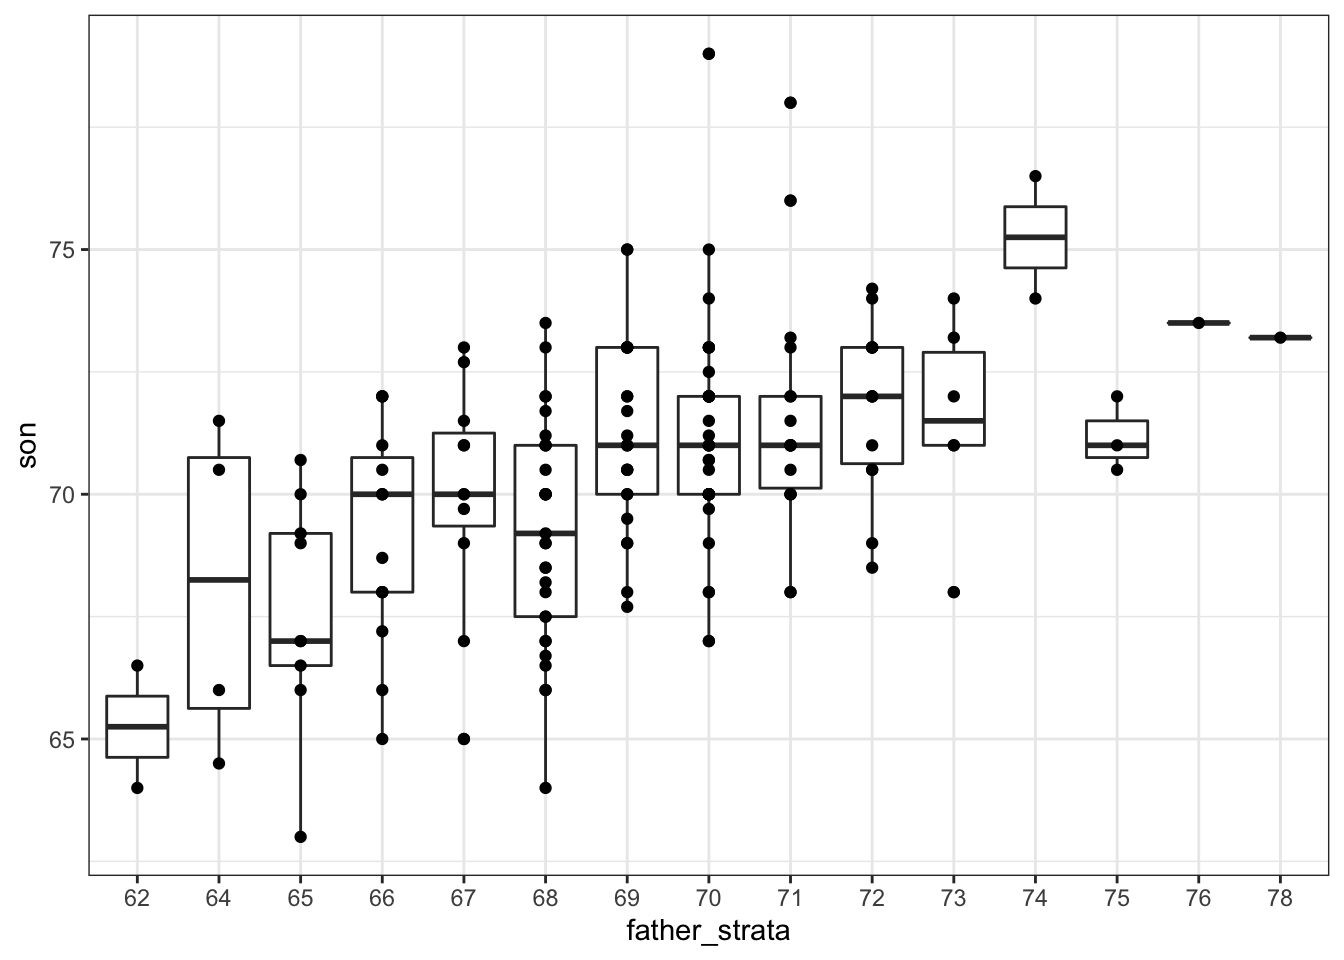
\includegraphics{Data_Science_Linear_Regression_files/figure-latex/unnamed-chunk-19-1.pdf}

\begin{Shaded}
\begin{Highlighting}[]
\CommentTok{\# center of each boxplot}
\NormalTok{galton\_heights }\OperatorTok{\%\textgreater{}\%}
\StringTok{    }\KeywordTok{mutate}\NormalTok{(}\DataTypeTok{father =} \KeywordTok{round}\NormalTok{(father)) }\OperatorTok{\%\textgreater{}\%}
\StringTok{    }\KeywordTok{group\_by}\NormalTok{(father) }\OperatorTok{\%\textgreater{}\%}
\StringTok{    }\KeywordTok{summarize}\NormalTok{(}\DataTypeTok{son\_conditional\_avg =} \KeywordTok{mean}\NormalTok{(son)) }\OperatorTok{\%\textgreater{}\%}
\StringTok{    }\KeywordTok{ggplot}\NormalTok{(}\KeywordTok{aes}\NormalTok{(father, son\_conditional\_avg)) }\OperatorTok{+}
\StringTok{    }\KeywordTok{geom\_point}\NormalTok{()}
\end{Highlighting}
\end{Shaded}

\begin{verbatim}
## `summarise()` ungrouping output (override with `.groups` argument)
\end{verbatim}

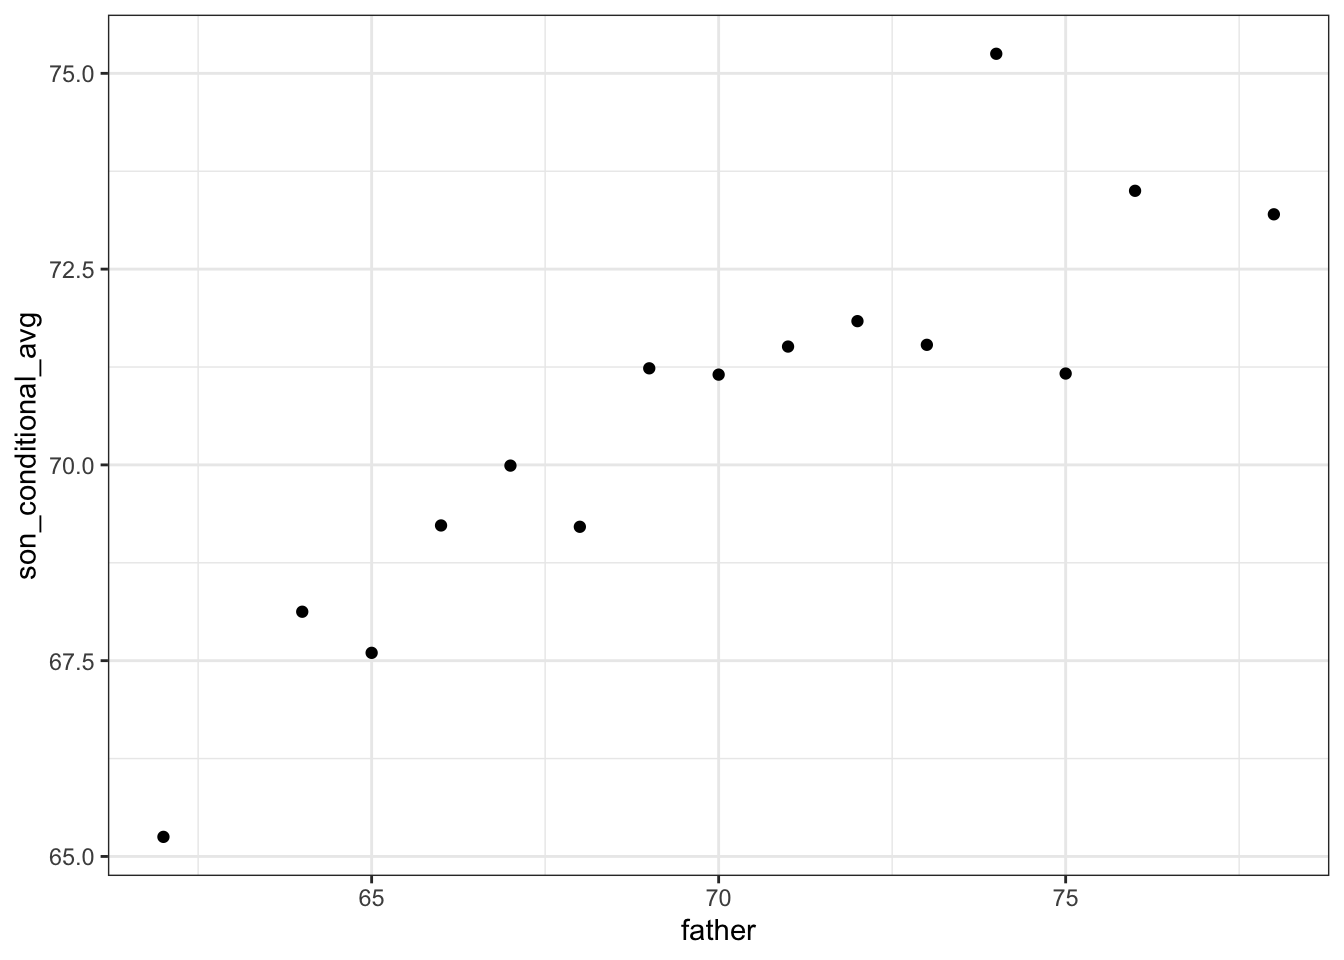
\includegraphics{Data_Science_Linear_Regression_files/figure-latex/unnamed-chunk-19-2.pdf}

\begin{Shaded}
\begin{Highlighting}[]
\CommentTok{\# calculate values to plot regression line on original data}
\NormalTok{mu\_x \textless{}{-}}\StringTok{ }\KeywordTok{mean}\NormalTok{(galton\_heights}\OperatorTok{$}\NormalTok{father)}
\NormalTok{mu\_y \textless{}{-}}\StringTok{ }\KeywordTok{mean}\NormalTok{(galton\_heights}\OperatorTok{$}\NormalTok{son)}
\NormalTok{s\_x \textless{}{-}}\StringTok{ }\KeywordTok{sd}\NormalTok{(galton\_heights}\OperatorTok{$}\NormalTok{father)}
\NormalTok{s\_y \textless{}{-}}\StringTok{ }\KeywordTok{sd}\NormalTok{(galton\_heights}\OperatorTok{$}\NormalTok{son)}
\NormalTok{r \textless{}{-}}\StringTok{ }\KeywordTok{cor}\NormalTok{(galton\_heights}\OperatorTok{$}\NormalTok{father, galton\_heights}\OperatorTok{$}\NormalTok{son)}
\NormalTok{m \textless{}{-}}\StringTok{ }\NormalTok{r }\OperatorTok{*}\StringTok{ }\NormalTok{s\_y}\OperatorTok{/}\NormalTok{s\_x}
\NormalTok{b \textless{}{-}}\StringTok{ }\NormalTok{mu\_y }\OperatorTok{{-}}\StringTok{ }\NormalTok{m}\OperatorTok{*}\NormalTok{mu\_x}

\CommentTok{\# add regression line to plot}
\NormalTok{galton\_heights }\OperatorTok{\%\textgreater{}\%}
\StringTok{    }\KeywordTok{ggplot}\NormalTok{(}\KeywordTok{aes}\NormalTok{(father, son)) }\OperatorTok{+}
\StringTok{    }\KeywordTok{geom\_point}\NormalTok{(}\DataTypeTok{alpha =} \FloatTok{0.5}\NormalTok{) }\OperatorTok{+}
\StringTok{    }\KeywordTok{geom\_abline}\NormalTok{(}\DataTypeTok{intercept =}\NormalTok{ b, }\DataTypeTok{slope =}\NormalTok{ m)}
\end{Highlighting}
\end{Shaded}

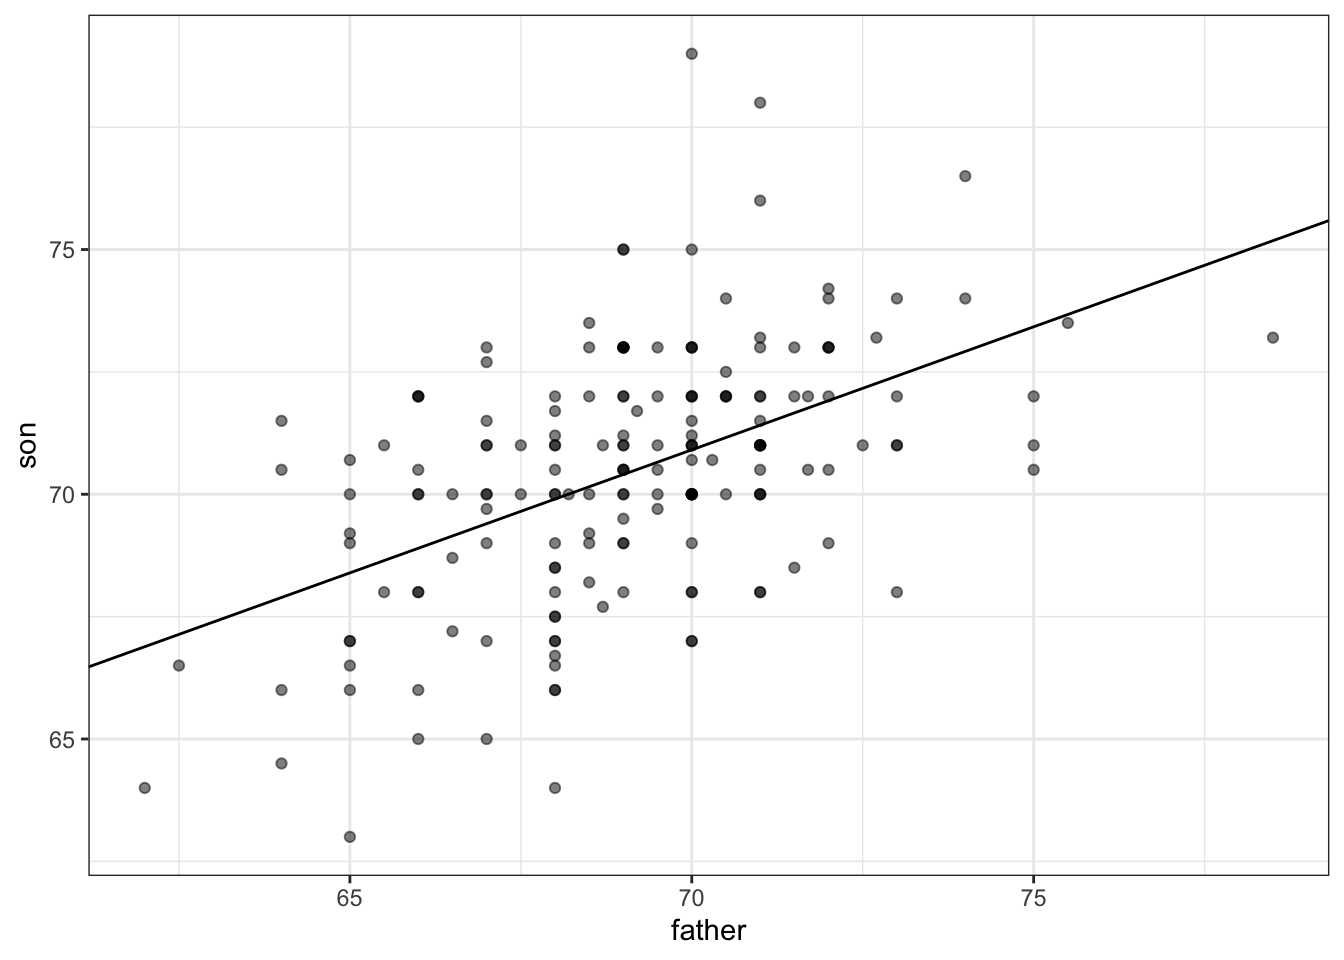
\includegraphics{Data_Science_Linear_Regression_files/figure-latex/unnamed-chunk-19-3.pdf}

\hypertarget{bivariate-normal-distribution}{%
\subsection{Bivariate Normal
Distribution}\label{bivariate-normal-distribution}}

There is a link to the relevant section of the textbook:
\href{https://rafalab.github.io/dsbook/regression.html\#bivariate-normal-distribution-advanced}{Bivariate
normal distribution (advanced)}

\textbf{Key points}

\begin{itemize}
\tightlist
\item
  When a pair of random variables are approximated by the bivariate
  normal distribution, scatterplots look like ovals. They can be thin
  (high correlation) or circle-shaped (no correlation).
\item
  When two variables follow a bivariate normal distribution, computing
  the regression line is equivalent to computing conditional
  expectations.
\item
  We can obtain a much more stable estimate of the conditional
  expectation by finding the regression line and using it to make
  predictions.
\end{itemize}

\emph{Code}

\begin{Shaded}
\begin{Highlighting}[]
\NormalTok{galton\_heights }\OperatorTok{\%\textgreater{}\%}
\StringTok{  }\KeywordTok{mutate}\NormalTok{(}\DataTypeTok{z\_father =} \KeywordTok{round}\NormalTok{((father }\OperatorTok{{-}}\StringTok{ }\KeywordTok{mean}\NormalTok{(father)) }\OperatorTok{/}\StringTok{ }\KeywordTok{sd}\NormalTok{(father))) }\OperatorTok{\%\textgreater{}\%}
\StringTok{  }\KeywordTok{filter}\NormalTok{(z\_father }\OperatorTok{\%in\%}\StringTok{ }\DecValTok{{-}2}\OperatorTok{:}\DecValTok{2}\NormalTok{) }\OperatorTok{\%\textgreater{}\%}
\StringTok{  }\KeywordTok{ggplot}\NormalTok{() }\OperatorTok{+}\StringTok{  }
\StringTok{  }\KeywordTok{stat\_qq}\NormalTok{(}\KeywordTok{aes}\NormalTok{(}\DataTypeTok{sample =}\NormalTok{ son)) }\OperatorTok{+}
\StringTok{  }\KeywordTok{facet\_wrap}\NormalTok{( }\OperatorTok{\textasciitilde{}}\StringTok{ }\NormalTok{z\_father)}
\end{Highlighting}
\end{Shaded}

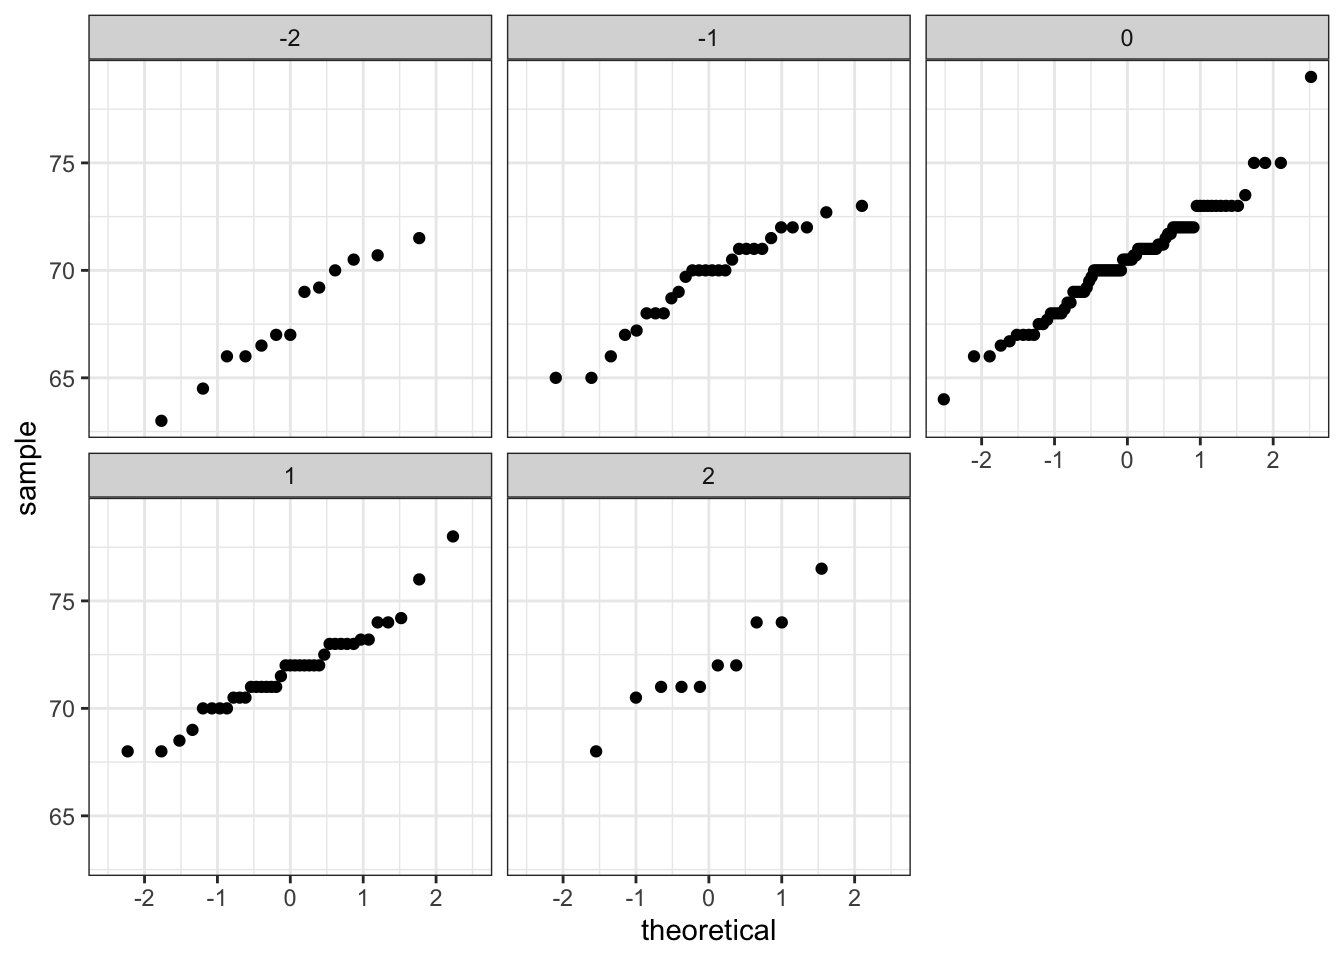
\includegraphics{Data_Science_Linear_Regression_files/figure-latex/unnamed-chunk-20-1.pdf}

\hypertarget{variance-explained}{%
\subsection{Variance Explained}\label{variance-explained}}

There is a link to the relevant section of the textbook:
\href{https://rafalab.github.io/dsbook/regression.html\#variance-explained}{Variance
explained}

\textbf{Key points}

\begin{itemize}
\tightlist
\item
  Conditioning on a random variable X can help to reduce variance of
  response variable Y.
\item
  The standard deviation of the conditional distribution is
  \(\mbox{SD}(Y \mid X=x) = \sigma_y\sqrt{1-\rho^2}\), which is smaller
  than the standard deviation without conditioning \(\sigma_y\).
\item
  Because variance is the standard deviation squared, the variance of
  the conditional distribution is \(\sigma_y^2(1-\rho^2)\).
\item
  In the statement ``X explains such and such percent of the
  variability,'' the percent value refers to the variance. The variance
  decreases by \(\rho^2\) percent.
\item
  The ``variance explained'' statement only makes sense when the data is
  approximated by a bivariate normal distribution.
\end{itemize}

\hypertarget{there-are-two-regression-lines}{%
\subsection{There are Two Regression
Lines}\label{there-are-two-regression-lines}}

There is a link to the relevant section of the textbook:
\href{https://rafalab.github.io/dsbook/regression.html\#warning-there-are-two-regression-lines}{Warning:
there are two regression lines}

\textbf{Key point}

There are two different regression lines depending on whether we are
taking the expectation of Y given X or taking the expectation of X given
Y.

\emph{Code}

\begin{Shaded}
\begin{Highlighting}[]
\CommentTok{\# compute a regression line to predict the son\textquotesingle{}s height from the father\textquotesingle{}s height}
\NormalTok{mu\_x \textless{}{-}}\StringTok{ }\KeywordTok{mean}\NormalTok{(galton\_heights}\OperatorTok{$}\NormalTok{father)}
\NormalTok{mu\_y \textless{}{-}}\StringTok{ }\KeywordTok{mean}\NormalTok{(galton\_heights}\OperatorTok{$}\NormalTok{son)}
\NormalTok{s\_x \textless{}{-}}\StringTok{ }\KeywordTok{sd}\NormalTok{(galton\_heights}\OperatorTok{$}\NormalTok{father)}
\NormalTok{s\_y \textless{}{-}}\StringTok{ }\KeywordTok{sd}\NormalTok{(galton\_heights}\OperatorTok{$}\NormalTok{son)}
\NormalTok{r \textless{}{-}}\StringTok{ }\KeywordTok{cor}\NormalTok{(galton\_heights}\OperatorTok{$}\NormalTok{father, galton\_heights}\OperatorTok{$}\NormalTok{son)}
\NormalTok{m\_}\DecValTok{1}\NormalTok{ \textless{}{-}}\StringTok{  }\NormalTok{r }\OperatorTok{*}\StringTok{ }\NormalTok{s\_y }\OperatorTok{/}\StringTok{ }\NormalTok{s\_x}
\NormalTok{b\_}\DecValTok{1}\NormalTok{ \textless{}{-}}\StringTok{ }\NormalTok{mu\_y }\OperatorTok{{-}}\StringTok{ }\NormalTok{m\_}\DecValTok{1}\OperatorTok{*}\NormalTok{mu\_x}

\CommentTok{\# compute a regression line to predict the father\textquotesingle{}s height from the son\textquotesingle{}s height}
\NormalTok{m\_}\DecValTok{2}\NormalTok{ \textless{}{-}}\StringTok{  }\NormalTok{r }\OperatorTok{*}\StringTok{ }\NormalTok{s\_x }\OperatorTok{/}\StringTok{ }\NormalTok{s\_y}
\NormalTok{b\_}\DecValTok{2}\NormalTok{ \textless{}{-}}\StringTok{ }\NormalTok{mu\_x }\OperatorTok{{-}}\StringTok{ }\NormalTok{m\_}\DecValTok{2}\OperatorTok{*}\NormalTok{mu\_y}
\end{Highlighting}
\end{Shaded}

\hypertarget{assessment---stratification-and-variance-explained-part-1}{%
\subsection{Assessment - Stratification and Variance Explained, Part
1}\label{assessment---stratification-and-variance-explained-part-1}}

\begin{enumerate}
\def\labelenumi{\arabic{enumi}.}
\tightlist
\item
  Look at the figure below. The slope of the regression line in this
  figure is equal to what, in words?
\end{enumerate}

\begin{figure}
\centering
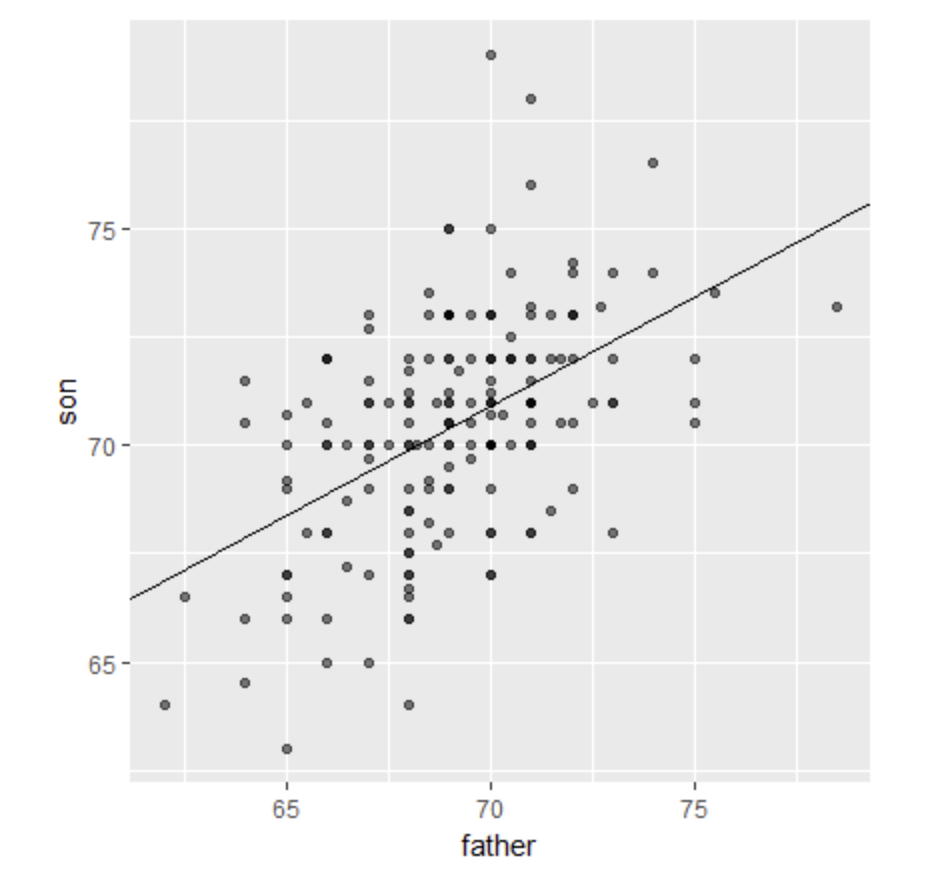
\includegraphics{images/regression_line_father_son.png}
\caption{Scatter plot and regression line of son and father heights}
\end{figure}

\begin{itemize}
\tightlist
\item[$\boxtimes$]
  A. Slope = (correlation coefficient of son and father heights) *
  (standard deviation of sons' heights / standard deviation of fathers'
  heights)
\item[$\square$]
  B. Slope = (correlation coefficient of son and father heights) *
  (standard deviation of fathers' heights / standard deviation of sons'
  heights)
\item[$\square$]
  C. Slope = (correlation coefficient of son and father heights) /
  (standard deviation of sons' heights * standard deviation of fathers'
  heights)
\item[$\square$]
  D. Slope = (mean height of fathers) - (correlation coefficient of son
  and father heights * mean height of sons).
\end{itemize}

\begin{enumerate}
\def\labelenumi{\arabic{enumi}.}
\setcounter{enumi}{1}
\tightlist
\item
  Why does the regression line simplify to a line with intercept zero
  and slope when we standardize our x and y variables? Try the
  simplification on your own first!
\end{enumerate}

\begin{itemize}
\tightlist
\item[$\square$]
  A. When we standardize variables, both x and y will have a mean of one
  and a standard deviation of zero. When you substitute this into the
  formula for the regression line, the terms cancel out until we have
  the following equation: \(y_i=px_i\).
\item[$\boxtimes$]
  B. When we standardize variables, both x and y will have a mean of
  zero and a standard deviation of one. When you substitute this into
  the formula for the regression line, the terms cancel out until we
  have the following equation: \(y_i = px_i\).
\item[$\square$]
  C. When we standardize variables, both x and y will have a mean of
  zero and a standard deviation of one. When you substitute this into
  the formula for the regression line, the terms cancel out until we
  have the following equation: \(y_i=px_i\).
\end{itemize}

\begin{enumerate}
\def\labelenumi{\arabic{enumi}.}
\setcounter{enumi}{2}
\tightlist
\item
  What is a limitation of calculating conditional means?
\end{enumerate}

\begin{itemize}
\tightlist
\item[$\boxtimes$]
  A. Each stratum we condition on (e.g., a specific father's height) may
  not have many data points.
\item[$\boxtimes$]
  B. Because there are limited data points for each stratum, our average
  values have large standard errors.
\item[$\boxtimes$]
  C. Conditional means are less stable than a regression line.
\item[$\square$]
  D. Conditional means are a useful theoretical tool but cannot be
  calculated.
\end{itemize}

\hypertarget{assessment-8---bivariate-normal-distribution}{%
\subsection{Assessment 8 - Bivariate Normal
Distribution}\label{assessment-8---bivariate-normal-distribution}}

\begin{enumerate}
\def\labelenumi{\arabic{enumi}.}
\tightlist
\item
  A regression line is the best prediction of Y given we know the value
  of X when:
\end{enumerate}

\begin{itemize}
\tightlist
\item[$\boxtimes$]
  A. X and Y follow a bivariate normal distribution.
\item[$\square$]
  B. Both X and Y are normally distributed.
\item[$\square$]
  C. Both X and Y have been standardized.
\item[$\square$]
  D. There are at least 25 X-Y pairs.
\end{itemize}

\begin{enumerate}
\def\labelenumi{\arabic{enumi}.}
\setcounter{enumi}{1}
\tightlist
\item
  Which one of the following scatterplots depicts an x and y
  distribution that is NOT well-approximated by the bivariate normal
  distribution?
\end{enumerate}

\begin{itemize}
\tightlist
\item[$\boxtimes$]
  A.
\end{itemize}

\begin{figure}
\centering
\includegraphics{https://user-images.githubusercontent.com/17474099/88281437-f64d6380-cce7-11ea-8401-dc487c96fcd8.png}
\caption{Scatter plot A}
\end{figure}

\begin{itemize}
\tightlist
\item[$\square$]
  B.
\end{itemize}

\begin{figure}
\centering
\includegraphics{https://user-images.githubusercontent.com/17474099/88281550-2dbc1000-cce8-11ea-8fbc-31d4a9f9baf3.png}
\caption{Scatter plot B}
\end{figure}

\begin{itemize}
\tightlist
\item[$\square$]
  C.
\end{itemize}

\begin{figure}
\centering
\includegraphics{https://user-images.githubusercontent.com/17474099/88281645-58a66400-cce8-11ea-9dfa-c39b2114ffa7.png}
\caption{Scatter plot C}
\end{figure}

\begin{itemize}
\tightlist
\item[$\square$]
  D.
\end{itemize}

\begin{figure}
\centering
\includegraphics{https://user-images.githubusercontent.com/17474099/88281807-986d4b80-cce8-11ea-9d0d-719572315c01.png}
\caption{Scatter plot D}
\end{figure}

\hypertarget{assessment-9---variance-explained}{%
\subsection{Assessment 9 - Variance
Explained}\label{assessment-9---variance-explained}}

\begin{enumerate}
\def\labelenumi{\arabic{enumi}.}
\tightlist
\item
  We previously calculated that the correlation coefficient between
  fathers' and sons' heights is 0.5.
\end{enumerate}

Given this, what percent of the variation in sons' heights is explained
by fathers' heights?

\begin{itemize}
\tightlist
\item[$\square$]
  A. 0\%
\item[$\boxtimes$]
  B. 25\%
\item[$\square$]
  C. 50\%
\item[$\square$]
  D. 75\%
\end{itemize}

\hypertarget{linear-models-overview}{%
\subsection{Linear Models Overview}\label{linear-models-overview}}

In the Linear Models section, you will learn how to do linear
regression.

After completing this section, you will be able to:

\begin{itemize}
\tightlist
\item
  Use multivariate regression to adjust for confounders.
\item
  Write linear models to describe the relationship between two or more
  variables.
\item
  Calculate the least squares estimates for a regression model using the
  lm function.
\item
  Understand the differences between tibbles and data frames.
\item
  Use the do function to bridge R functions and the tidyverse.
\item
  Use the tidy, glance, and augment functions from the broom package.
\item
  Apply linear regression to measurement error models.
\end{itemize}

This section has four parts: Introduction to Linear Models, Least
Squares Estimates, Tibbles, do, and broom, and Regression and Baseball.

The textbook for this section is available
\href{https://rafalab.github.io/dsbook/linear-models.html\#confounding}{here}

\hypertarget{assessment-1---confounding-are-bbs-more-predictive}{%
\subsection{Assessment 1 - Confounding: Are BBs More
Predictive?}\label{assessment-1---confounding-are-bbs-more-predictive}}

\begin{enumerate}
\def\labelenumi{\arabic{enumi}.}
\tightlist
\item
  Why is the number of home runs considered a confounder of the
  relationship between bases on balls and runs per game?
\end{enumerate}

\begin{itemize}
\tightlist
\item[$\square$]
  A. Home runs is not a confounder of this relationship.
\item[$\square$]
  B. Home runs are the primary cause of runs per game.
\item[$\square$]
  C. The correlation between home runs and runs per game is stronger
  than the correlation between bases on balls and runs per game.
\item[$\boxtimes$]
  D. Players who get more bases on balls also tend to have more home
  runs; in addition, home runs increase the points per game.
\end{itemize}

\hypertarget{assessment-2---stratification-and-multivariate-regression}{%
\subsection{Assessment 2 - Stratification and Multivariate
Regression}\label{assessment-2---stratification-and-multivariate-regression}}

\begin{enumerate}
\def\labelenumi{\arabic{enumi}.}
\tightlist
\item
  As described in the video, when we stratified our regression lines for
  runs per game vs.~bases on balls by the number of home runs, what
  happened?
\end{enumerate}

\begin{itemize}
\tightlist
\item[$\boxtimes$]
  A. The slope of runs per game vs.~bases on balls within each stratum
  was reduced because we removed confounding by home runs.
\item[$\square$]
  B. The slope of runs per game vs.~bases on balls within each stratum
  was reduced because there were fewer data points.
\item[$\square$]
  C. The slope of runs per game vs.~bases on balls within each stratum
  increased after we removed confounding by home runs.
\item[$\square$]
  D. The slope of runs per game vs.~bases on balls within each stratum
  stayed about the same as the original slope.
\end{itemize}

\hypertarget{assessment-3---linear-models}{%
\subsection{Assessment 3 - Linear
Models}\label{assessment-3---linear-models}}

\begin{enumerate}
\def\labelenumi{\arabic{enumi}.}
\tightlist
\item
  We run a linear model for sons' heights vs.~fathers' heights using the
  Galton height data, and get the following results:
\end{enumerate}

\begin{Shaded}
\begin{Highlighting}[]
\OperatorTok{\textgreater{}}\StringTok{ }\KeywordTok{lm}\NormalTok{(son }\OperatorTok{\textasciitilde{}}\StringTok{ }\NormalTok{father, }\DataTypeTok{data =}\NormalTok{ galton\_heights)}

\NormalTok{Call}\OperatorTok{:}
\KeywordTok{lm}\NormalTok{(}\DataTypeTok{formula =}\NormalTok{ son }\OperatorTok{\textasciitilde{}}\StringTok{ }\NormalTok{father, }\DataTypeTok{data =}\NormalTok{ galton\_heights)}

\NormalTok{Coefficients}\OperatorTok{:}
\NormalTok{(Intercept)    father  }
    \FloatTok{35.71}       \FloatTok{0.50}  
\end{Highlighting}
\end{Shaded}

Interpret the numeric coefficient for ``father.''

\begin{itemize}
\tightlist
\item[$\square$]
  A. For every inch we increase the son's height, the predicted father's
  height increases by 0.5 inches.
\item[$\boxtimes$]
  B. For every inch we increase the father's height, the predicted son's
  height grows by 0.5 inches.
\item[$\square$]
  C. For every inch we increase the father's height, the predicted son's
  height is 0.5 times greater.
\end{itemize}

\begin{enumerate}
\def\labelenumi{\arabic{enumi}.}
\setcounter{enumi}{1}
\tightlist
\item
  We want the intercept term for our model to be more interpretable, so
  we run the same model as before but now we subtract the mean of
  fathers' heights from each individual father's height to create a new
  variable centered at zero.
\end{enumerate}

\begin{Shaded}
\begin{Highlighting}[]
\NormalTok{galton\_heights \textless{}{-}}\StringTok{ }\NormalTok{galton\_heights }\OperatorTok{\%\textgreater{}\%}
\StringTok{    }\KeywordTok{mutate}\NormalTok{(}\DataTypeTok{father\_centered=}\NormalTok{father }\OperatorTok{{-}}\StringTok{ }\KeywordTok{mean}\NormalTok{(father))}
\end{Highlighting}
\end{Shaded}

We run a linear model using this centered fathers' height variable.

\begin{Shaded}
\begin{Highlighting}[]
\OperatorTok{\textgreater{}}\StringTok{ }\KeywordTok{lm}\NormalTok{(son }\OperatorTok{\textasciitilde{}}\StringTok{ }\NormalTok{father\_centered, }\DataTypeTok{data =}\NormalTok{ galton\_heights)}

\NormalTok{Call}\OperatorTok{:}
\KeywordTok{lm}\NormalTok{(}\DataTypeTok{formula =}\NormalTok{ son }\OperatorTok{\textasciitilde{}}\StringTok{ }\NormalTok{father\_centered, }\DataTypeTok{data =}\NormalTok{ galton\_heights)}

\NormalTok{Coefficients}\OperatorTok{:}
\NormalTok{(Intercept)    father\_centered  }
    \FloatTok{70.45}          \FloatTok{0.50}  
\end{Highlighting}
\end{Shaded}

Interpret the numeric coefficient for the intercept.

\begin{itemize}
\tightlist
\item[$\boxtimes$]
  A. The height of a son of a father of average height is 70.45 inches.
\item[$\square$]
  B. The height of a son when a father's height is zero is 70.45 inches.
\item[$\square$]
  C. The height of an average father is 70.45 inches.
\end{itemize}

\hypertarget{assessment-4---least-squares-estimates-lse}{%
\subsection{Assessment 4 - Least Squares Estimates
(LSE)}\label{assessment-4---least-squares-estimates-lse}}

\begin{enumerate}
\def\labelenumi{\arabic{enumi}.}
\tightlist
\item
  The following code was used in the video to plot RSS with
  \(\beta_0=25\).
\end{enumerate}

\begin{Shaded}
\begin{Highlighting}[]
\NormalTok{beta1 =}\StringTok{ }\KeywordTok{seq}\NormalTok{(}\DecValTok{0}\NormalTok{, }\DecValTok{1}\NormalTok{, }\DataTypeTok{len=}\KeywordTok{nrow}\NormalTok{(galton\_heights))}
\NormalTok{results \textless{}{-}}\StringTok{ }\KeywordTok{data.frame}\NormalTok{(}\DataTypeTok{beta1 =}\NormalTok{ beta1,}
                      \DataTypeTok{rss =} \KeywordTok{sapply}\NormalTok{(beta1, rss, }\DataTypeTok{beta0 =} \DecValTok{25}\NormalTok{))}
\NormalTok{results }\OperatorTok{\%\textgreater{}\%}\StringTok{ }\KeywordTok{ggplot}\NormalTok{(}\KeywordTok{aes}\NormalTok{(beta1, rss)) }\OperatorTok{+}\StringTok{ }\KeywordTok{geom\_line}\NormalTok{() }\OperatorTok{+}\StringTok{ }
\StringTok{  }\KeywordTok{geom\_line}\NormalTok{(}\KeywordTok{aes}\NormalTok{(beta1, rss), }\DataTypeTok{col=}\DecValTok{2}\NormalTok{)}
\end{Highlighting}
\end{Shaded}

In a model for sons' heights vs fathers' heights, what is the least
squares estimate (LSE) for \(\beta_1\) if we assume \(\hat{\beta}_{0}\)
is 36?

\begin{itemize}
\tightlist
\item[$\square$]
  A. 0.65
\item[$\boxtimes$]
  B. 0.5
\item[$\square$]
  C. 0.2
\item[$\square$]
  D. 12
\end{itemize}

\begin{enumerate}
\def\labelenumi{\arabic{enumi}.}
\setcounter{enumi}{1}
\tightlist
\item
  The least squares estimates for the parameters
  \(\beta_1,\beta_2...\beta_n\) \textbf{minimize} the residual sum of
  squares.
\end{enumerate}

\hypertarget{assessment-5---the-lm-function}{%
\subsection{Assessment 5 - The lm
Function}\label{assessment-5---the-lm-function}}

\begin{enumerate}
\def\labelenumi{\arabic{enumi}.}
\tightlist
\item
  Run a linear model in R predicting the number of runs per game based
  on the number of bases on balls and the number of home runs. Remember
  to first limit your data to 1961-2001.
\end{enumerate}

What is the coefficient for bases on balls?

\begin{itemize}
\tightlist
\item[$\boxtimes$]
  A. 0.39
\item[$\square$]
  B. 1.56
\item[$\square$]
  C. 1.74
\item[$\square$]
  D. 0.027
\end{itemize}

\hypertarget{assessment-6---lse-are-random-variables}{%
\subsection{Assessment 6 - LSE are Random
Variables}\label{assessment-6---lse-are-random-variables}}

\begin{enumerate}
\def\labelenumi{\arabic{enumi}.}
\tightlist
\item
  We run a Monte Carlo simulation where we repeatedly take samples of N
  = 100 from the Galton heights data and compute the regression slope
  coefficients for each sample:
\end{enumerate}

\begin{Shaded}
\begin{Highlighting}[]
\NormalTok{B \textless{}{-}}\StringTok{ }\DecValTok{1000}
\NormalTok{N \textless{}{-}}\StringTok{ }\DecValTok{100}
\NormalTok{lse \textless{}{-}}\StringTok{ }\KeywordTok{replicate}\NormalTok{(B, \{}
  \KeywordTok{sample\_n}\NormalTok{(galton\_heights, N, }\DataTypeTok{replace =} \OtherTok{TRUE}\NormalTok{) }\OperatorTok{\%\textgreater{}\%}\StringTok{ }
\StringTok{    }\KeywordTok{lm}\NormalTok{(son }\OperatorTok{\textasciitilde{}}\StringTok{ }\NormalTok{father, }\DataTypeTok{data =}\NormalTok{ .) }\OperatorTok{\%\textgreater{}\%}\StringTok{ }\NormalTok{.}\OperatorTok{$}\NormalTok{coef }
\NormalTok{\})}

\NormalTok{lse \textless{}{-}}\StringTok{ }\KeywordTok{data.frame}\NormalTok{(}\DataTypeTok{beta\_0 =}\NormalTok{ lse[}\DecValTok{1}\NormalTok{,], }\DataTypeTok{beta\_1 =}\NormalTok{ lse[}\DecValTok{2}\NormalTok{,]) }
\end{Highlighting}
\end{Shaded}

What does the central limit theorem tell us about the variables beta\_0
and beta\_1?

\begin{itemize}
\tightlist
\item[$\boxtimes$]
  A. They are approximately normally distributed.
\item[$\boxtimes$]
  B. The expected value of each is the true value of \(\beta_0\) and
  \(\beta_1\) (assuming the Galton heights data is a complete
  population).
\item[$\square$]
  C. The central limit theorem does not apply in this situation.
\item[$\square$]
  D. It allows us to test the hypothesis that \(\beta_0=0\) and
  \(\beta_0=1\)
\end{itemize}

\begin{enumerate}
\def\labelenumi{\arabic{enumi}.}
\setcounter{enumi}{1}
\tightlist
\item
  In an earlier video, we ran the following linear model and looked at a
  summary of the results.
\end{enumerate}

\begin{Shaded}
\begin{Highlighting}[]
\OperatorTok{$}\NormalTok{\textbackslash{}beta\_}\DecValTok{0} \OperatorTok{$}
\ErrorTok{\textgreater{}}\StringTok{ }\NormalTok{mod \textless{}{-}}\StringTok{ }\KeywordTok{lm}\NormalTok{(son }\OperatorTok{\textasciitilde{}}\StringTok{ }\NormalTok{father, }\DataTypeTok{data =}\NormalTok{ galton\_heights)}
\OperatorTok{\textgreater{}}\StringTok{ }\KeywordTok{summary}\NormalTok{(mod)}

\NormalTok{Call}\OperatorTok{:}
\KeywordTok{lm}\NormalTok{(}\DataTypeTok{formula =}\NormalTok{ son }\OperatorTok{\textasciitilde{}}\StringTok{ }\NormalTok{father, }\DataTypeTok{data =}\NormalTok{ galton\_heights)}

\NormalTok{Residuals}\OperatorTok{:}
\StringTok{   }\NormalTok{Min     1Q  Median     3Q    Max }
\FloatTok{{-}5.902}  \FloatTok{{-}1.405}  \FloatTok{0.092}    \FloatTok{1.342}  \FloatTok{8.092} 

\NormalTok{Coefficients}\OperatorTok{:}
\StringTok{                 }\NormalTok{Estimate  Std. Error  t value     }\KeywordTok{Pr}\NormalTok{(}\OperatorTok{\textgreater{}}\ErrorTok{|}\NormalTok{t}\OperatorTok{|}\NormalTok{)  }
\NormalTok{(Intercept)     }\FloatTok{35.7125}     \FloatTok{4.5174}       \FloatTok{7.91}    \FloatTok{2.8e{-}13} \OperatorTok{**}\ErrorTok{*}
\NormalTok{father           }\FloatTok{0.5028}     \FloatTok{0.0653}       \FloatTok{7.70}    \FloatTok{9.5e{-}13} \OperatorTok{**}\ErrorTok{*}
\OperatorTok{{-}{-}{-}}
\NormalTok{Signif. codes}\OperatorTok{:}\StringTok{  }\DecValTok{0}\NormalTok{ ‘}\OperatorTok{**}\ErrorTok{*}\NormalTok{’ }\FloatTok{0.001}\NormalTok{ ‘}\OperatorTok{**}\NormalTok{’ }\FloatTok{0.01}\NormalTok{ ‘}\OperatorTok{*}\NormalTok{’ }\FloatTok{0.05}\NormalTok{ ‘.’ }\FloatTok{0.1}\NormalTok{ ‘ ’ }\DecValTok{1}
\OperatorTok{$}\NormalTok{\textbackslash{}beta\_}\DecValTok{0} \OperatorTok{$}
\end{Highlighting}
\end{Shaded}

What null hypothesis is the second p-value (the one in the father row)
testing?

\begin{itemize}
\tightlist
\item[$\square$]
  A. \(\beta_1 = 1\), where \(\beta_1\) is the coefficient for the
  variable ``father.''
\item[$\square$]
  B. \(\beta_1 = 0.503\), where \(\beta_1\) is the coefficient for the
  variable ``father.''
\item[$\boxtimes$]
  C. \(\beta_1 = 0\), where \(\beta_1\) is the coefficient for the
  variable ``father.''
\end{itemize}

\hypertarget{assessment-7---predicted-variables-are-random-variables}{%
\subsection{Assessment 7 - Predicted Variables are Random
Variables}\label{assessment-7---predicted-variables-are-random-variables}}

\begin{enumerate}
\def\labelenumi{\arabic{enumi}.}
\tightlist
\item
  Which R code(s) below would properly plot the predictions and
  confidence intervals for our linear model of sons' heights?
\end{enumerate}

\begin{itemize}
\tightlist
\item[$\square$]
  A.
\end{itemize}

\begin{Shaded}
\begin{Highlighting}[]
\NormalTok{galton\_heights }\OperatorTok{\%\textgreater{}\%}\StringTok{ }\KeywordTok{ggplot}\NormalTok{(}\KeywordTok{aes}\NormalTok{(father, son)) }\OperatorTok{+}
\StringTok{  }\KeywordTok{geom\_point}\NormalTok{() }\OperatorTok{+}
\StringTok{  }\KeywordTok{geom\_smooth}\NormalTok{()}
\end{Highlighting}
\end{Shaded}

\begin{itemize}
\tightlist
\item[$\boxtimes$]
  B.
\end{itemize}

\begin{Shaded}
\begin{Highlighting}[]
\NormalTok{galton\_heights }\OperatorTok{\%\textgreater{}\%}\StringTok{ }\KeywordTok{ggplot}\NormalTok{(}\KeywordTok{aes}\NormalTok{(father, son)) }\OperatorTok{+}
\StringTok{  }\KeywordTok{geom\_point}\NormalTok{() }\OperatorTok{+}
\StringTok{  }\KeywordTok{geom\_smooth}\NormalTok{(}\DataTypeTok{method =} \StringTok{"lm"}\NormalTok{)}
\end{Highlighting}
\end{Shaded}

\begin{itemize}
\tightlist
\item[$\boxtimes$]
  C.
\end{itemize}

\begin{Shaded}
\begin{Highlighting}[]
\NormalTok{model \textless{}{-}}\StringTok{ }\KeywordTok{lm}\NormalTok{(son }\OperatorTok{\textasciitilde{}}\StringTok{ }\NormalTok{father, }\DataTypeTok{data =}\NormalTok{ galton\_heights)}
\NormalTok{predictions \textless{}{-}}\StringTok{ }\KeywordTok{predict}\NormalTok{(model, }\DataTypeTok{interval =} \KeywordTok{c}\NormalTok{(}\StringTok{"confidence"}\NormalTok{), }\DataTypeTok{level =} \FloatTok{0.95}\NormalTok{)}
\NormalTok{data \textless{}{-}}\StringTok{ }\KeywordTok{as.tibble}\NormalTok{(predictions) }\OperatorTok{\%\textgreater{}\%}\StringTok{ }\KeywordTok{bind\_cols}\NormalTok{(}\DataTypeTok{father =}\NormalTok{ galton\_heights}\OperatorTok{$}\NormalTok{father)}

\KeywordTok{ggplot}\NormalTok{(data, }\KeywordTok{aes}\NormalTok{(}\DataTypeTok{x =}\NormalTok{ father, }\DataTypeTok{y =}\NormalTok{ fit)) }\OperatorTok{+}
\StringTok{  }\KeywordTok{geom\_line}\NormalTok{(}\DataTypeTok{color =} \StringTok{"blue"}\NormalTok{, }\DataTypeTok{size =} \DecValTok{1}\NormalTok{) }\OperatorTok{+}\StringTok{ }
\StringTok{  }\KeywordTok{geom\_ribbon}\NormalTok{(}\KeywordTok{aes}\NormalTok{(}\DataTypeTok{ymin=}\NormalTok{lwr, }\DataTypeTok{ymax=}\NormalTok{upr), }\DataTypeTok{alpha=}\FloatTok{0.2}\NormalTok{) }\OperatorTok{+}\StringTok{ }
\StringTok{  }\KeywordTok{geom\_point}\NormalTok{(}\DataTypeTok{data =}\NormalTok{ galton\_heights, }\KeywordTok{aes}\NormalTok{(}\DataTypeTok{x =}\NormalTok{ father, }\DataTypeTok{y =}\NormalTok{ son))}
\end{Highlighting}
\end{Shaded}

\begin{itemize}
\tightlist
\item[$\square$]
  D.
\end{itemize}

\begin{Shaded}
\begin{Highlighting}[]
\NormalTok{model \textless{}{-}}\StringTok{ }\KeywordTok{lm}\NormalTok{(son }\OperatorTok{\textasciitilde{}}\StringTok{ }\NormalTok{father, }\DataTypeTok{data =}\NormalTok{ galton\_heights)}
\NormalTok{predictions \textless{}{-}}\StringTok{ }\KeywordTok{predict}\NormalTok{(model)}
\NormalTok{data \textless{}{-}}\StringTok{ }\KeywordTok{as.tibble}\NormalTok{(predictions) }\OperatorTok{\%\textgreater{}\%}\StringTok{ }\KeywordTok{bind\_cols}\NormalTok{(}\DataTypeTok{father =}\NormalTok{ galton\_heights}\OperatorTok{$}\NormalTok{father)}

\KeywordTok{ggplot}\NormalTok{(data, }\KeywordTok{aes}\NormalTok{(}\DataTypeTok{x =}\NormalTok{ father, }\DataTypeTok{y =}\NormalTok{ fit)) }\OperatorTok{+}
\StringTok{  }\KeywordTok{geom\_line}\NormalTok{(}\DataTypeTok{color =} \StringTok{"blue"}\NormalTok{, }\DataTypeTok{size =} \DecValTok{1}\NormalTok{) }\OperatorTok{+}\StringTok{ }
\StringTok{  }\KeywordTok{geom\_point}\NormalTok{(}\DataTypeTok{data =}\NormalTok{ galton\_heights, }\KeywordTok{aes}\NormalTok{(}\DataTypeTok{x =}\NormalTok{ father, }\DataTypeTok{y =}\NormalTok{ son))}
\end{Highlighting}
\end{Shaded}

\hypertarget{assessment-8---advanced-dplyr-tibbles}{%
\subsection{Assessment 8 - Advanced dplyr:
Tibbles}\label{assessment-8---advanced-dplyr-tibbles}}

\begin{enumerate}
\def\labelenumi{\arabic{enumi}.}
\tightlist
\item
  What problem do we encounter when we try to run a linear model on our
  baseball data, grouping by home runs?
\end{enumerate}

\begin{itemize}
\tightlist
\item[$\square$]
  A. There is not enough data in some levels to run the model.
\item[$\boxtimes$]
  B. The \texttt{lm} function does not know how to handle grouped
  tibbles.
\item[$\square$]
  C. The results of the \texttt{lm} function cannot be put into a tidy
  format.
\end{itemize}

\begin{enumerate}
\def\labelenumi{\arabic{enumi}.}
\setcounter{enumi}{1}
\tightlist
\item
  Tibbles are similar to what other class in R?
\end{enumerate}

\begin{itemize}
\tightlist
\item[$\square$]
  A. Vectors
\item[$\square$]
  B. Matrices
\item[$\boxtimes$]
  C. Data frames
\item[$\square$]
  D. Lists
\end{itemize}

\hypertarget{assessment-9---tibbles-differences-from-data-frames}{%
\subsection{Assessment 9 - Tibbles: Differences from Data
Frames}\label{assessment-9---tibbles-differences-from-data-frames}}

\begin{enumerate}
\def\labelenumi{\arabic{enumi}.}
\tightlist
\item
  What are some advantages of tibbles compared to data frames?
\end{enumerate}

\begin{itemize}
\tightlist
\item[$\boxtimes$]
  A. Tibbles display better.
\item[$\boxtimes$]
  B. If you subset a tibble, you always get back a tibble.
\item[$\boxtimes$]
  C. Tibbles can have complex entries.
\item[$\boxtimes$]
  D. Tibbles can be grouped.
\end{itemize}

\hypertarget{assessment-10---do}{%
\subsection{Assessment 10 - do}\label{assessment-10---do}}

\begin{enumerate}
\def\labelenumi{\arabic{enumi}.}
\tightlist
\item
  What are two advantages of the do command, when applied to the
  tidyverse?
\end{enumerate}

\begin{itemize}
\tightlist
\item[$\square$]
  A. It is faster than normal functions.
\item[$\square$]
  B. It returns useful error messages.
\item[$\boxtimes$]
  C. It understands grouped tibbles.
\item[$\boxtimes$]
  D. It always returns a data.frame.
\end{itemize}

\begin{enumerate}
\def\labelenumi{\arabic{enumi}.}
\setcounter{enumi}{1}
\tightlist
\item
  You want to take the tibble dat, which we've been using in this video,
  and run the linear model R \textasciitilde{} BB for each strata of HR.
  Then you want to add three new columns to your grouped tibble: the
  coefficient, standard error, and p-value for the BB term in the model.
\end{enumerate}

You've already written the function \texttt{get\_slope}, shown below.

\begin{Shaded}
\begin{Highlighting}[]
\NormalTok{get\_slope \textless{}{-}}\StringTok{ }\ControlFlowTok{function}\NormalTok{(data) \{}
\NormalTok{  fit \textless{}{-}}\StringTok{ }\KeywordTok{lm}\NormalTok{(R }\OperatorTok{\textasciitilde{}}\StringTok{ }\NormalTok{BB, }\DataTypeTok{data =}\NormalTok{ data)}
\NormalTok{  sum.fit \textless{}{-}}\StringTok{ }\KeywordTok{summary}\NormalTok{(fit)}

  \KeywordTok{data.frame}\NormalTok{(}\DataTypeTok{slope =}\NormalTok{ sum.fit}\OperatorTok{$}\NormalTok{coefficients[}\DecValTok{2}\NormalTok{, }\StringTok{"Estimate"}\NormalTok{], }
             \DataTypeTok{se =}\NormalTok{ sum.fit}\OperatorTok{$}\NormalTok{coefficients[}\DecValTok{2}\NormalTok{, }\StringTok{"Std. Error"}\NormalTok{],}
             \DataTypeTok{pvalue =}\NormalTok{ sum.fit}\OperatorTok{$}\NormalTok{coefficients[}\DecValTok{2}\NormalTok{, }\StringTok{"Pr(\textgreater{}|t|)"}\NormalTok{])}
\NormalTok{\}}
\end{Highlighting}
\end{Shaded}

What additional code could you write to accomplish your goal?

\begin{itemize}
\tightlist
\item[$\square$]
  A.
\end{itemize}

\begin{Shaded}
\begin{Highlighting}[]
\NormalTok{dat }\OperatorTok{\%\textgreater{}\%}\StringTok{ }
\StringTok{  }\KeywordTok{group\_by}\NormalTok{(HR) }\OperatorTok{\%\textgreater{}\%}\StringTok{ }
\StringTok{  }\KeywordTok{do}\NormalTok{(get\_slope)}
\end{Highlighting}
\end{Shaded}

\begin{itemize}
\tightlist
\item[$\boxtimes$]
  B.
\end{itemize}

\begin{Shaded}
\begin{Highlighting}[]
\NormalTok{dat }\OperatorTok{\%\textgreater{}\%}\StringTok{ }
\StringTok{  }\KeywordTok{group\_by}\NormalTok{(HR) }\OperatorTok{\%\textgreater{}\%}\StringTok{ }
\StringTok{  }\KeywordTok{do}\NormalTok{(}\KeywordTok{get\_slope}\NormalTok{(.))}
\end{Highlighting}
\end{Shaded}

\begin{itemize}
\tightlist
\item[$\square$]
  C.
\end{itemize}

\begin{Shaded}
\begin{Highlighting}[]
\NormalTok{dat }\OperatorTok{\%\textgreater{}\%}\StringTok{ }
\StringTok{  }\KeywordTok{group\_by}\NormalTok{(HR) }\OperatorTok{\%\textgreater{}\%}\StringTok{ }
\StringTok{  }\KeywordTok{do}\NormalTok{(}\DataTypeTok{slope =} \KeywordTok{get\_slope}\NormalTok{(.))}
\end{Highlighting}
\end{Shaded}

\begin{itemize}
\tightlist
\item[$\square$]
  D.
\end{itemize}

\begin{Shaded}
\begin{Highlighting}[]
\NormalTok{dat }\OperatorTok{\%\textgreater{}\%}\StringTok{ }
\StringTok{  }\KeywordTok{do}\NormalTok{(}\KeywordTok{get\_slope}\NormalTok{(.))}
\end{Highlighting}
\end{Shaded}

\hypertarget{assessment-11---broom}{%
\subsection{Assessment 11 - broom}\label{assessment-11---broom}}

\begin{enumerate}
\def\labelenumi{\arabic{enumi}.}
\tightlist
\item
  The output of a broom function is always what?
\end{enumerate}

\begin{itemize}
\tightlist
\item[$\boxtimes$]
  A. A data.frame
\item[$\square$]
  B. A list
\item[$\square$]
  C. A vector
\end{itemize}

\begin{enumerate}
\def\labelenumi{\arabic{enumi}.}
\setcounter{enumi}{1}
\tightlist
\item
  You want to know whether the relationship between home runs and runs
  per game varies by baseball league. You create the following dataset:
\end{enumerate}

\begin{Shaded}
\begin{Highlighting}[]
\NormalTok{dat \textless{}{-}}\StringTok{ }\NormalTok{Teams }\OperatorTok{\%\textgreater{}\%}\StringTok{ }\KeywordTok{filter}\NormalTok{(yearID }\OperatorTok{\%in\%}\StringTok{ }\DecValTok{1961}\OperatorTok{:}\DecValTok{2001}\NormalTok{) }\OperatorTok{\%\textgreater{}\%}
\StringTok{  }\KeywordTok{mutate}\NormalTok{(}\DataTypeTok{HR =}\NormalTok{ HR}\OperatorTok{/}\NormalTok{G,}
         \DataTypeTok{R =}\NormalTok{ R}\OperatorTok{/}\NormalTok{G) }\OperatorTok{\%\textgreater{}\%}
\StringTok{  }\KeywordTok{select}\NormalTok{(lgID, HR, BB, R)}
\end{Highlighting}
\end{Shaded}

What code would help you quickly answer this question?

\begin{itemize}
\tightlist
\item[$\boxtimes$]
  A.
\end{itemize}

\begin{Shaded}
\begin{Highlighting}[]
\NormalTok{dat }\OperatorTok{\%\textgreater{}\%}\StringTok{ }
\StringTok{  }\KeywordTok{group\_by}\NormalTok{(lgID) }\OperatorTok{\%\textgreater{}\%}\StringTok{ }
\StringTok{  }\KeywordTok{do}\NormalTok{(}\KeywordTok{tidy}\NormalTok{(}\KeywordTok{lm}\NormalTok{(R }\OperatorTok{\textasciitilde{}}\StringTok{ }\NormalTok{HR, }\DataTypeTok{data =}\NormalTok{ .), }\DataTypeTok{conf.int =}\NormalTok{ T)) }\OperatorTok{\%\textgreater{}\%}\StringTok{ }
\StringTok{  }\KeywordTok{filter}\NormalTok{(term }\OperatorTok{==}\StringTok{ "HR"}\NormalTok{)}
\end{Highlighting}
\end{Shaded}

\begin{itemize}
\tightlist
\item[$\square$]
  B.
\end{itemize}

\begin{Shaded}
\begin{Highlighting}[]
\NormalTok{dat }\OperatorTok{\%\textgreater{}\%}\StringTok{ }
\StringTok{  }\KeywordTok{group\_by}\NormalTok{(lgID) }\OperatorTok{\%\textgreater{}\%}\StringTok{ }
\StringTok{  }\KeywordTok{do}\NormalTok{(}\KeywordTok{glance}\NormalTok{(}\KeywordTok{lm}\NormalTok{(R }\OperatorTok{\textasciitilde{}}\StringTok{ }\NormalTok{HR, }\DataTypeTok{data =}\NormalTok{ .)))}
\end{Highlighting}
\end{Shaded}

\begin{itemize}
\tightlist
\item[$\square$]
  C.
\end{itemize}

\begin{Shaded}
\begin{Highlighting}[]
\NormalTok{dat }\OperatorTok{\%\textgreater{}\%}\StringTok{ }
\StringTok{  }\KeywordTok{do}\NormalTok{(}\KeywordTok{tidy}\NormalTok{(}\KeywordTok{lm}\NormalTok{(R }\OperatorTok{\textasciitilde{}}\StringTok{ }\NormalTok{HR, }\DataTypeTok{data =}\NormalTok{ .), }\DataTypeTok{conf.int =}\NormalTok{ T)) }\OperatorTok{\%\textgreater{}\%}\StringTok{ }
\StringTok{  }\KeywordTok{filter}\NormalTok{(term }\OperatorTok{==}\StringTok{ "HR"}\NormalTok{)}
\end{Highlighting}
\end{Shaded}

\begin{itemize}
\tightlist
\item[$\square$]
  D.
\end{itemize}

\begin{Shaded}
\begin{Highlighting}[]
\NormalTok{dat }\OperatorTok{\%\textgreater{}\%}\StringTok{ }
\StringTok{  }\KeywordTok{group\_by}\NormalTok{(lgID) }\OperatorTok{\%\textgreater{}\%}\StringTok{ }
\StringTok{  }\KeywordTok{do}\NormalTok{(}\DataTypeTok{mod =} \KeywordTok{lm}\NormalTok{(R }\OperatorTok{\textasciitilde{}}\StringTok{ }\NormalTok{HR, }\DataTypeTok{data =}\NormalTok{ .))}
\end{Highlighting}
\end{Shaded}

\hypertarget{assessment-12---building-a-better-offensive-metric-for-baseball}{%
\subsection{Assessment 12 - Building a Better Offensive Metric for
Baseball}\label{assessment-12---building-a-better-offensive-metric-for-baseball}}

\begin{enumerate}
\def\labelenumi{\arabic{enumi}.}
\tightlist
\item
  What is the final linear model we use to predict runs scored per game?
\end{enumerate}

\begin{itemize}
\tightlist
\item[$\square$]
  A. \texttt{lm(R\ \textasciitilde{}\ BB\ +\ HR)}
\item[$\square$]
  B.
  \texttt{lm(HR\ \textasciitilde{}\ BB\ +\ singles\ +\ doubles\ +\ triples)}
\item[$\boxtimes$]
  C.
  \texttt{lm(R\ \textasciitilde{}\ BB\ +\ singles\ +\ doubles\ +\ triples\ +\ HR)}
\item[$\square$]
  D.
  \texttt{lm(R\ \textasciitilde{}\ singles\ +\ doubles\ +\ triples\ +\ HR)}
\end{itemize}

\begin{enumerate}
\def\labelenumi{\arabic{enumi}.}
\setcounter{enumi}{1}
\tightlist
\item
  We want to estimate runs per game scored by individual players, not
  just by teams. What summary metric do we calculate to help estimate
  this?
\end{enumerate}

Look at the code from the video for a hint:

\begin{Shaded}
\begin{Highlighting}[]
\NormalTok{pa\_per\_game \textless{}{-}}\StringTok{ }\NormalTok{Batting }\OperatorTok{\%\textgreater{}\%}\StringTok{ }
\StringTok{  }\KeywordTok{filter}\NormalTok{(yearID }\OperatorTok{==}\StringTok{ }\DecValTok{2002}\NormalTok{) }\OperatorTok{\%\textgreater{}\%}\StringTok{ }
\StringTok{  }\KeywordTok{group\_by}\NormalTok{(teamID) }\OperatorTok{\%\textgreater{}\%}
\StringTok{  }\KeywordTok{summarize}\NormalTok{(}\DataTypeTok{pa\_per\_game =} \KeywordTok{sum}\NormalTok{(AB}\OperatorTok{+}\NormalTok{BB)}\OperatorTok{/}\KeywordTok{max}\NormalTok{(G)) }\OperatorTok{\%\textgreater{}\%}\StringTok{ }
\StringTok{  }\NormalTok{.}\OperatorTok{$}\NormalTok{pa\_per\_game }\OperatorTok{\%\textgreater{}\%}\StringTok{ }
\StringTok{  }\NormalTok{mean}
\end{Highlighting}
\end{Shaded}

\begin{itemize}
\tightlist
\item[$\square$]
  A. \texttt{pa\_per\_game}: the mean number of plate appearances per
  team per game for each team
\item[$\square$]
  B. \texttt{pa\_per\_game}: the mean number of plate appearances per
  game for each player
\item[$\boxtimes$]
  C. \texttt{pa\_per\_game}: the number of plate appearances per team
  per game, averaged across all teams
\end{itemize}

\begin{enumerate}
\def\labelenumi{\arabic{enumi}.}
\setcounter{enumi}{2}
\tightlist
\item
  Imagine you have two teams. Team A is comprised of batters who, on
  average, get two bases on balls, four singles, one double, and one
  home run. Team B is comprised of batters who, on average, get one base
  on balls, six singles, two doubles, and one triple.
\end{enumerate}

Which team scores more runs, as predicted by our model?

\begin{itemize}
\tightlist
\item[$\square$]
  A. Team A
\item[$\boxtimes$]
  B. Team B
\item[$\square$]
  C. Tie
\item[$\square$]
  D. Impossible to know
\end{itemize}

\hypertarget{assessment-13---on-base-plus-slugging-ops}{%
\subsection{Assessment 13 - On Base Plus Slugging
(OPS)}\label{assessment-13---on-base-plus-slugging-ops}}

\begin{enumerate}
\def\labelenumi{\arabic{enumi}.}
\tightlist
\item
  The on-base-percentage plus slugging percentage (OPS) metric gives the
  most weight to:
\end{enumerate}

\begin{itemize}
\tightlist
\item[$\square$]
  A. Singles
\item[$\square$]
  B. Doubles
\item[$\square$]
  C. Triples
\item[$\boxtimes$]
  D. Home Runs
\end{itemize}

\hypertarget{assessment-14---regression-fallacy}{%
\subsection{Assessment 14 - Regression
Fallacy}\label{assessment-14---regression-fallacy}}

\begin{enumerate}
\def\labelenumi{\arabic{enumi}.}
\tightlist
\item
  What statistical concept properly explains the ``sophomore slump''?
\end{enumerate}

\begin{itemize}
\tightlist
\item[$\boxtimes$]
  A. Regression to the mean
\item[$\square$]
  B. Law of averages
\item[$\square$]
  C. Normal distribution
\end{itemize}

\hypertarget{assessment-15---measurement-error-models}{%
\subsection{Assessment 15 - Measurement Error
Models}\label{assessment-15---measurement-error-models}}

\begin{enumerate}
\def\labelenumi{\arabic{enumi}.}
\tightlist
\item
  In our model of time vs.~observed\_distance, the randomness of our
  data was due to:
\end{enumerate}

\begin{itemize}
\tightlist
\item[$\square$]
  A. sampling
\item[$\square$]
  B. natural variability
\item[$\boxtimes$]
  C. measurement error
\end{itemize}

\begin{enumerate}
\def\labelenumi{\arabic{enumi}.}
\setcounter{enumi}{1}
\tightlist
\item
  Which of the following are important assumptions about the measurement
  errors in this experiment?
\end{enumerate}

\begin{itemize}
\tightlist
\item[$\boxtimes$]
  A. The measurement error is random
\item[$\boxtimes$]
  B. The measurement error is independent
\item[$\boxtimes$]
  C. The measurement error has the same distribution for each time i
\end{itemize}

\begin{enumerate}
\def\labelenumi{\arabic{enumi}.}
\setcounter{enumi}{2}
\tightlist
\item
  Which of the following scenarios would violate an assumption of our
  measurement error model?
\end{enumerate}

\begin{itemize}
\tightlist
\item[$\square$]
  A. The experiment was conducted on the moon.
\item[$\boxtimes$]
  B. There was one position where it was particularly difficult to see
  the dropped ball.
\item[$\square$]
  C. The experiment was only repeated 10 times, not 100 times.
\end{itemize}

\hypertarget{confounding-overview}{%
\subsection{Confounding Overview}\label{confounding-overview}}

In the Confounding section, you will learn what is perhaps the most
important lesson of statistics: that correlation is not causation.

After completing this section, you will be able to:

\begin{itemize}
\tightlist
\item
  Identify examples of spurious correlation and explain how data
  dredging can lead to spurious correlation.
\item
  Explain how outliers can drive correlation and learn to adjust for
  outliers using Spearman correlation.
\item
  Explain how reversing cause and effect can lead to associations being
  confused with causation.
\item
  Understand how confounders can lead to the misinterpretation of
  associations.
\item
  Explain and give examples of Simpson's Paradox.
\end{itemize}

This section has one part: Correlation is Not Causation.

The textbook for this section is available
\href{https://rafalab.github.io/dsbook/association-is-not-causation.html}{here}

\hypertarget{assessment-1---correlation-is-not-causation-spurious-correlation}{%
\subsection{Assessment 1 - Correlation is Not Causation: Spurious
Correlation}\label{assessment-1---correlation-is-not-causation-spurious-correlation}}

\begin{enumerate}
\def\labelenumi{\arabic{enumi}.}
\tightlist
\item
  In the video, we ran one million tests of correlation for two random
  variables, X and Y.
\end{enumerate}

How many of these correlations would you expect to have a significant
p-value (p\textgreater0.05), just by chance?

\begin{itemize}
\tightlist
\item[$\square$]
  A. 5,000
\item[$\boxtimes$]
  B. 50,000
\item[$\square$]
  C. 100,000
\item[$\square$]
  D. It's impossible to know
\end{itemize}

\begin{enumerate}
\def\labelenumi{\arabic{enumi}.}
\setcounter{enumi}{1}
\tightlist
\item
  Which of the following are examples of p-hacking?
\end{enumerate}

\begin{itemize}
\tightlist
\item[$\boxtimes$]
  A. Looking for associations between an outcome and several exposures
  and only reporting the one that is significant.
\item[$\boxtimes$]
  B. Trying several different models and selecting the one that yields
  the smallest p-value.
\item[$\boxtimes$]
  C. Repeating an experiment multiple times and only reporting the one
  with the smallest p-value.
\item[$\square$]
  D. Using a Monte Carlo simulations in an analysis.
\end{itemize}

\hypertarget{assessment-2---correlation-is-not-causation-outliers}{%
\subsection{Assessment 2 - Correlation is Not Causation:
Outliers}\label{assessment-2---correlation-is-not-causation-outliers}}

\begin{enumerate}
\def\labelenumi{\arabic{enumi}.}
\tightlist
\item
  The Spearman correlation coefficient is robust to outliers because:
\end{enumerate}

\begin{itemize}
\tightlist
\item[$\square$]
  A. It drops outliers before calculating correlation.
\item[$\square$]
  B. It is the correlation of standardized values.
\item[$\boxtimes$]
  C. It calculates correlation between ranks, not values.
\end{itemize}

\hypertarget{assessment-3---correlation-is-not-causation-reversing-cause-and-effect}{%
\subsection{Assessment 3 - Correlation is Not Causation: Reversing Cause
and
Effect}\label{assessment-3---correlation-is-not-causation-reversing-cause-and-effect}}

\begin{enumerate}
\def\labelenumi{\arabic{enumi}.}
\tightlist
\item
  Which of the following may be examples of reversed cause and effect?
\end{enumerate}

\begin{itemize}
\tightlist
\item[$\boxtimes$]
  A. Past smokers who have quit smoking may be more likely to die from
  lung cancer.
\item[$\square$]
  B. Tall fathers are more likely to have tall sons.
\item[$\boxtimes$]
  C. People with high blood pressure tend to have a healthier diet.
\item[$\boxtimes$]
  D. Individuals in a low social status have a higher risk of
  schizophrenia.
\end{itemize}

\hypertarget{assessment-4---correlation-is-not-causation-confounders}{%
\subsection{Assessment 4 - Correlation is Not Causation:
Confounders}\label{assessment-4---correlation-is-not-causation-confounders}}

\begin{enumerate}
\def\labelenumi{\arabic{enumi}.}
\tightlist
\item
  What can you do to determine if you are misinterpreting results
  because of a confounder?
\end{enumerate}

\begin{itemize}
\tightlist
\item[$\square$]
  A. Nothing, if the p-value says the result is significant, then it is.
\item[$\boxtimes$]
  B. More closely examine the results by stratifying and plotting the
  data.
\item[$\square$]
  C. Always assume that you are misinterpreting the results.
\item[$\square$]
  D. Use linear models to tease out a confounder.
\end{itemize}

\begin{enumerate}
\def\labelenumi{\arabic{enumi}.}
\setcounter{enumi}{1}
\tightlist
\item
  Look again at the admissions data using ?admissions. What important
  characteristic of the table variables do you need to know to
  understand the calculations used in this video? Select the best
  answer.
\end{enumerate}

\begin{itemize}
\tightlist
\item[$\square$]
  A. The data is from 1973.
\item[$\square$]
  B. The columns ``major'' and ``gender'' are of class character, while
  ``admitted'' and ``applicants'' are numeric.
\item[$\square$]
  C. The data is from the ``dslabs'' package.
\item[$\boxtimes$]
  D. The column ``admitted'' is the percent of student admitted, while
  the column ``applicants'' is the total number of applicants.
\end{itemize}

\begin{enumerate}
\def\labelenumi{\arabic{enumi}.}
\setcounter{enumi}{2}
\tightlist
\item
  In the example in the video, major selectivity confounds the
  relationship between UC Berkley admission rates and gender because:
\end{enumerate}

\begin{itemize}
\tightlist
\item[$\square$]
  A. It was harder for women to be admitted to UC Berkeley.
\item[$\boxtimes$]
  B. Major selectivity is associated with both admission rates and with
  gender, as women tended to apply to more selective majors.
\item[$\square$]
  C. Some majors are more selective than others
\item[$\square$]
  D. Major selectivity is not a confounder.
\end{itemize}

\hypertarget{assessment-5---simpsons-paradox}{%
\subsection{Assessment 5 - Simpson's
Paradox}\label{assessment-5---simpsons-paradox}}

\begin{enumerate}
\def\labelenumi{\arabic{enumi}.}
\tightlist
\item
  Admission rates at UC Berkeley are an example of Simpson's Paradox
  because:
\end{enumerate}

\begin{itemize}
\tightlist
\item[$\boxtimes$]
  A. It appears that men have higher a higher admission rate than women,
  however, after we stratify by major, we see that on average women have
  a higher admission rate than men.
\item[$\square$]
  B. It was a paradox that women were being admitted at a lower rate
  than men.
\item[$\square$]
  C. The relationship between admissions and gender is confounded by
  major selectivity.
\end{itemize}

\end{document}
